% !TeX spellcheck = de_AT_frami
\section{Grundlagen der Informatik}
In diesem Kapitel verschaffen wir uns einen groben Überblick zu grundlegenden Begrifflichkeiten aus der Informatik:
\begin{itemize}
	\item Hardwarekomponenten und Bootvorgang.
	\item Betriebssystem:  Wie wird die Hardware eines Computers dem Benutzer zur Anwendung nutzbar gemacht?
	\item Funktionsweise von Computernetzwerken, IPv4 und Konzepte wie das Client-Server-Modell.
	\item Virtualisierung: Virtuelle Maschinen, Container, virtuelle Netzwerke (VPN).
\end{itemize}
Die Inhalte sind fast baugleich entnommen aus den Lehrbüchern \cite{gumm3} und \cite{gumm2}, dem Lernmaterial des \link{https://learning.lpi.org/de/learning-materials/010-160/4/4.2/4.2_01/}{Linux Professional Institute} und teilweise \link{https://wikipedia.org}{Wikipedia}.

%
%
%
\subsection{Hardwarekomponenten}
%~\\
\begin{itemize}
	\item Aus Benutzersicht präsentiert sich der Computer (Stand-PC, Laptop, Tablet, Smartphone, Fahrradcomputer,...) über die Anwendungssoftware (\textit{apps}), die wir auf ihm ausführen und verwenden.
	\item Hardware verarbeitet die von der Software beschriebenen Befehle und stellt Mechanismen für Speicherung sowie Eingabe und Ausgabe bereit.
	\item Damit überhaupt eine Software auf einer bestimmten Hardware läuft, müssen geeignete Schnittstellen festgelegt werden; siehe dazu auch Abb. \ref{fig:betriebssystem}:
	%
	\begin{figure}[h!]
		\centering
		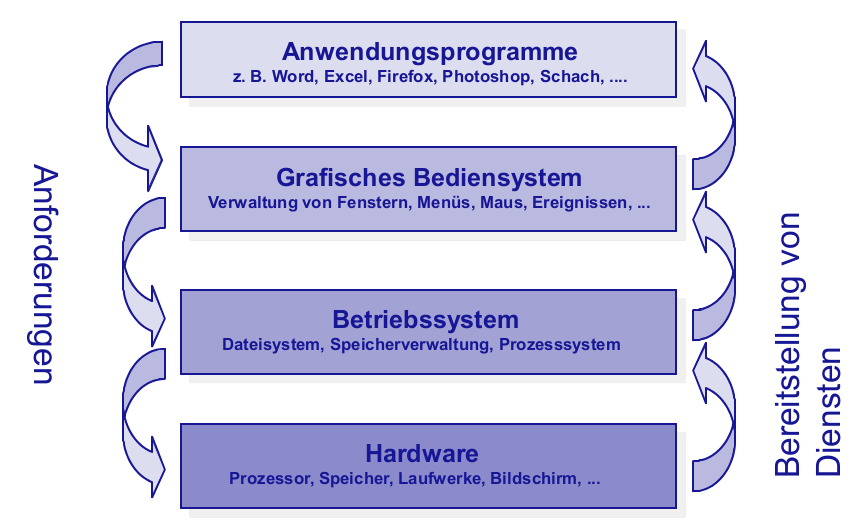
\includegraphics[width=0.5\linewidth]{./media/betriebssystem}
		\caption[Schnittstellen]{Zwischen diesen Schichten müssen geeignete Schnittstellen definiert und implementiert werden. Quelle: \cite[Abb. 1.25]{gumm2}}
		\label{fig:betriebssystem}
	\end{figure}
	%
\end{itemize}
%
Wir schauen uns einige Hardwarekomponenten als eigenständige physische Geräte und deren Standardschnittstellen genauer an. Die Standards sind relativ statisch, aber Form (Größe, Anschlüsse,...), Leistung (Zugriffsgeschwindigkeiten, Taktfrequenz,...) und Kapazität (Speichergröße,...) der Hardware entwickeln sich ständig weiter.

~\\
%NETZTEILE
\begin{minipage}[t]{0.7\textwidth}
	\subsubsection{Netzteile}
	\begin{itemize}
		\item Alle aktiven Komponenten in einem Computersystem benötigen zum Betrieb Strom.
		\item Netzteile normalisieren verfügbare Energiequellen.
		\item Standardisierte Spannungsanforderungen ermöglichen es Herstellern, Hardwarekomponenten zu entwickeln, die auf vielen Systemen laufen.
		\item Bei der Nutzung von Strom entsteht Wärme, die abgeführt wird durch:
		\begin{itemize}
			\item Ventilator (erzeugt Luftstrom, am Netzteil und anderen Komponenten)
			\item Kühlkörper (Rippenstruktur) mit guter Wärmeleitfähigkeit zur Vergrößerung der Oberfläche (Wärmeleitung an die Luft, welche dann über konvektiven Einfluss des Ventilators abgeführt werden kann)
		\end{itemize}
	\end{itemize}
\end{minipage}
\begin{minipage}[t]{0.3\textwidth}
	\centering
	~\\
	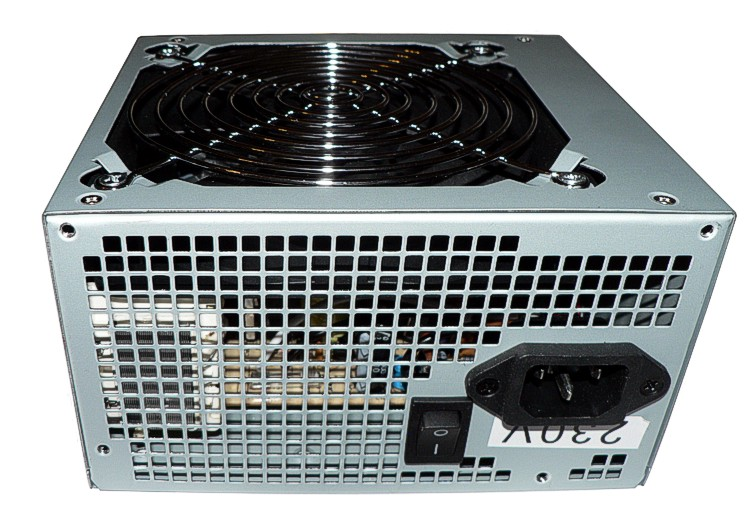
\includegraphics[width=1\linewidth]{./media/netzteil}\\
	\tiny
	Quelle: \url{https://de.wikipedia.org/wiki/PC-Netzteil}
\end{minipage}

%HAUPTPLATINE
\subsubsection{Hauptplatine (Motherboard) und Bootvorgang}
	\begin{figure}[h!]
		\centering
		~\\~\\
		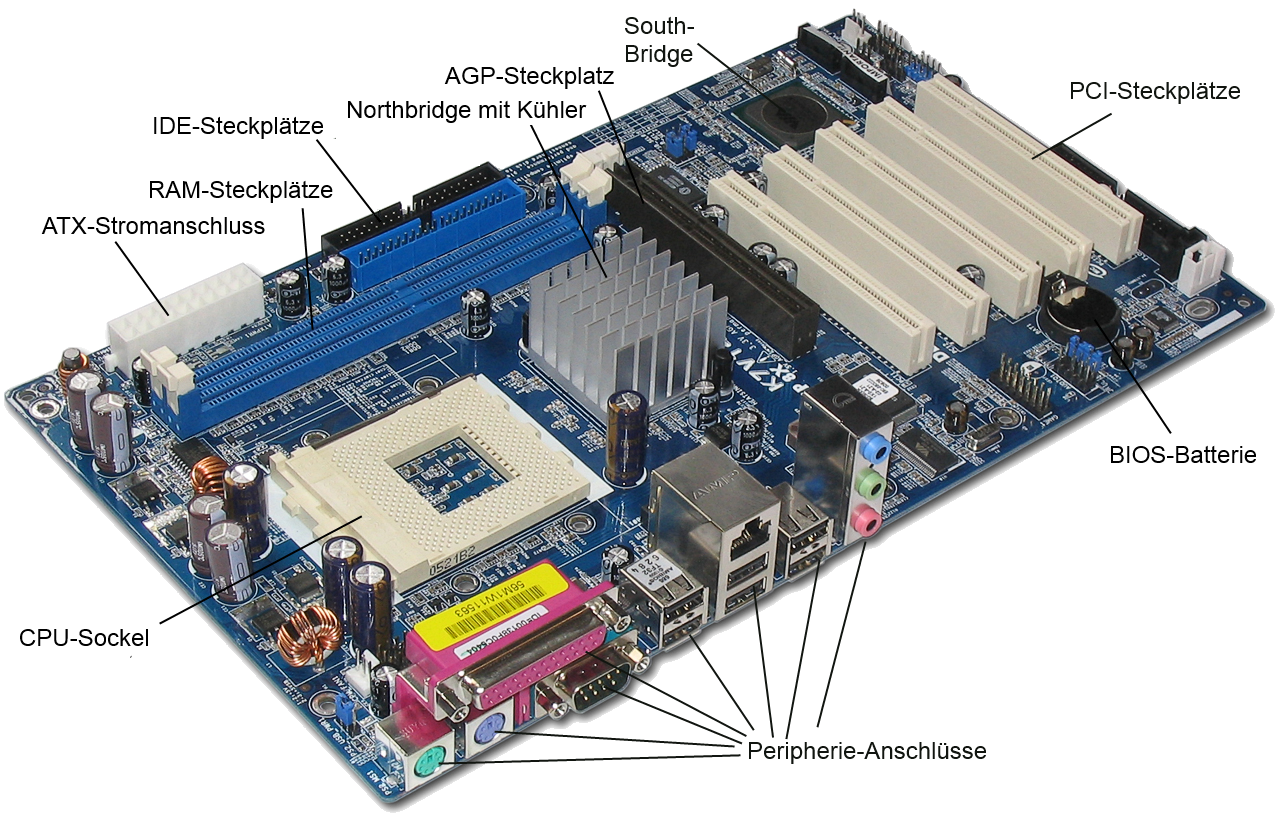
\includegraphics[width=0.5\linewidth]{./media/motherboard} \\
		\caption[Hauptplatine]{Hauptplatine. Quelle: https://de.wikipedia.org/wiki/Hauptplatine}
	\end{figure}
	\begin{itemize}
		\item Sämtliche Hardware eines Systems muss miteinander verbunden sein. Die Hauptplatine (auch \textit{Motherboard} oder \textit{Mainboard} genannt) normiert diese Verbindung mit standardisierten Steckverbindungen und Formfaktoren.
		\item Wird die Stromversorgung eingeschaltet, muss die mainboardspezifische Hardware konfiguriert und initialisiert werden, bevor das System laufen kann. Motherboards laden dazu Programme aus einem nichtflüchtigen Speicher (=bleibt erhalten unabhängig von Stromzufuhr), die als \textbf{\textit{Firmware}} oder \textbf{\textit{Basis--Software}} (\cite[2.1]{gumm2}) bezeichnet werden. Dabei handelt es sich noch nicht um Teile eines Betriebssystems.
		\item Zunächst werden u.a. die Komponenten des Rechners (CPU, Peripheriegeräte,...) getestet. Sind keine Fehler aufgetreten, wird von der Festplatte oder einem anderen Laufwerk das Betriebssystem geladen; man spricht bei diesem Vorgang von \textbf{booten}\footnote{Da ein Computer während des Bootvorgangs schon ein Programm lädt, das er zum Funktionieren benötigt, zieht er sich bildlich gesprochen wie Münchhausen an den eigenen Haaren aus dem Sumpf; die englischen Redewendung dazu: an seinen Stiefelriemen (engl. bootstraps) selbst über einen Zaun.}.
	\end{itemize}
%
~\\
In diesem Zusammenhang gibt es zwei wichtige Begriffe:
\begin{itemize}
	\item \textbf{BIOS}
\begin{itemize}
	\item Die ursprüngliche Form der Motherboard-Firmware wurde als BIOS (Basic Input/Output System) bezeichnet.
	\item Aufgaben: Grundlegende Konfigurationseinstellungen sowie die Identifizierung, das Laden und die Übertragung des Betriebs auf ein Betriebssystem wie Linux.
\end{itemize}
\item \textbf{UEFI}
\begin{itemize}
	\item Im Laufe der rasanten Hardwareentwicklung wurde auch die Firmware erweitert: Um größere Festplatten, Diagnosewerkzeuge, grafische Oberflächen, Netzwerke, usw.
	\item Mit dem Ziel die Schnittstelle zwischen Platinen--Firmware und Betriebssystem zu standardisieren wurde das Unified Extensible Firmware Interface (kurz UEFI, englisch für Vereinheitlichte erweiterbare Firmware-Schnittstelle) entwickelt (angeregt von Intel Ende der 90er mit EFI und vereinheitlicht zu UEFI von einem Konsortium von PC-Herstellern in 2006).
	\item UEFI hat sich als Nachfolger des BIOS etabliert und wird heute von den meisten Motherboards verwendet.
\end{itemize}
\end{itemize}
Unabhängig davon bezeichnen viele die Firmware des Motherboards immer noch als BIOS.
~\\~\\
\textbf{Der Bootvorgang} (mit UEFI)
\begin{enumerate}
	\item UEFI-kompatible Firmware des Motherboards (oft einfach als \textit{UEFI} bezeichnet) wird ausgeführt. Je nach Hersteller kann dabei ein optionales \textbf{Einstellungsmenü (\textbf{Bootmenü})} durch Drücken einer (F--)Funktionstasten eingeblendet werden. In der Praxis meist von Nöten, wenn man einen Rechner ``neu aufsetzen'' oder inspizieren möchte und dazu die Bootreihenfolge ändern muss (um ein Betriebssystem-Image von einem USB-Stick zu laden).
	\item Dann wird nach einem UEFI-kompatiblen \textbf{Bootloader} gesucht. Ein Bootloader (manchmal auch \textbf{Bootmanager} genannt) ist eine spezielle Software, die gewöhnlich durch die Firmware des Motherboards von einem wechselbaren veränderlichen Datenspeicher geladen und anschließend ausgeführt wird. Der Bootloader ist meist das erste Programm, das nach der unveränderlichen Firmware von einem wechselbaren veränderlichen Datenspeicher geladen wird.\\~\\
	Beispiel für Linux und weitere unixoide Betriebssysteme:\\ \textbf{Grand Unified Bootloader} (kurz \textbf{GRUB}, \textit{Großer vereinheitlichter Bootloader}), aktuell \textbf{GRUB2}.
\item Der Bootloader lädt dann weitere Teile des Betriebssystems, gewöhnlich einen Kernel. Es können mehrere Betriebssysteme zur Verfügung stehen. In diesem Fall erscheint meist ein Prompt\footnote{\hyperref{https://de.wikipedia.org/wiki/Prompt}{}{}{https://de.wikipedia.org/wiki/Prompt}: Als englisch prompt wird in der IT eine Aufforderung an den Benutzer bezeichnet, eine Eingabe (input) zu tätigen.}, welches den Benutzer auffordert eine Auswahl zu treffen. Damit können erweiterte Funktionen und unterschiedliche Startmodi realisiert werden.
\end{enumerate}
\clearpage
\demo{~\\
	\texttt{UEFI firmware (Motherboard) [Einstellungsmenü]}\\
	\texttt{> boot/efi/<distro>/grubx64.efi (Datenspeicher) [Bootmenü mit Kernelauswahl]} \\
	\texttt{> kernel }
	~\\~\\
	Unter Linux (hier Ubuntu):
	\begin{itemize}
		\item Der einfachste Weg herauszufinden, ob UEFI oder BIOS verwendet wird, ist nachzuschauen, ob das Verzeichnis $$\ttt{/sys/firmware/efi}$$
		vorhanden ist.
		\item Auf mordernen Systemen befindet sich der Bootloader dann auf der EFI (Extensible Firmware Interface) system partition (ESP), welche als $$\texttt{/boot/efi}$$ eingehangen wird; siehe zum Beispiel $$\texttt{\$ lsblk}.$$
		\item Die UEFI Firmware des Motherboard startet dann die Datei $$\texttt{boot/efi/<distro>/grubx64.efi} ~~~\text{(für x64 UEFI System)}.$$
		\item Die Konfiguration des GRUB finden wir in der Datei $$\texttt{/boot/grub/grub.cfg}$$
		wo ein Eintrag beispielsweise den Kernel aufruft:
		$$
		\texttt{linux	/boot/vmlinuz-5.11.0-44-generic root=UUID=(...) ro  \$vt\_handoff}
		$$
		Die Datei wird automatisch erzeugt mit den Einstellungen aus
		$$\texttt{/etc/default/grub}, $$
		mit Einträgen wie
		$$\texttt{GRUB\_CMDLINE\_LINUX\_DEFAULT=''quiet splash''},$$
		die wir besser zu
		$$\texttt{GRUB\_CMDLINE\_LINUX\_DEFAULT=''''}$$
		setzen, um einen gesprächigen Bootvorgang zu beobachten.
		\item Im Verzeichnis \texttt{/boot} finden wir den Link auf den Kernel
		$$\texttt{vmlinuz-5.11.0-44-generic}$$
\end{itemize}}



%SYSTEMSPEICHER (RAM)
	\subsubsection{Arbeitsspeicher (RAM)}
	\begin{itemize}
		\item Der Arbeitsspeicher enthält die Daten und den Programmcode der aktuell laufenden Anwendungen.
		\item Physisch gesehen wird der Arbeitsspeicher in der Regel auf einzelnen Platinenmodulen aufgebracht, die in das Motherboard eingesteckt werden.
		\item  4 GB ist für die meisten Standardanwendungen der minimale Arbeitsspeicher.
		\item Swap Space: Was geschieht, wenn eine Anwendung mehr als den verfügbaren Arbeitsspeicher benötigt? In diesem Fall verschiebt Linux ungenutzte Anwendungen aus dem Arbeitsspeicher in einen speziellen Plattenbereich, den Swap Space, und ungenutzte Anwendungen aus dem Swap Space zurück in den Arbeitsspeicher, wenn sie ausgeführt werden müssen.
	\end{itemize}
\demo{
	Unter Linux: Wie viel Speicherplatz steht zur Verfügung?
\begin{itemize}
	\item Für einen Benutzer ist üblicherweise die Gesamtmenge des verfügbaren und des verwendeten Speichers von Interesse. Eine Informationsquelle ist die Ausführung des Befehls $$\texttt{\$ free}$$ mit dem Parameter -m (oder -g) zur Ausgabe der Werte in Megabytes (oder Gigabytes).
\end{itemize}
}
%
%
%PROZESSOR
~\\
\subsubsection{Prozessor und CPU}
\begin{figure}[h!]
	\centering
	~\\
	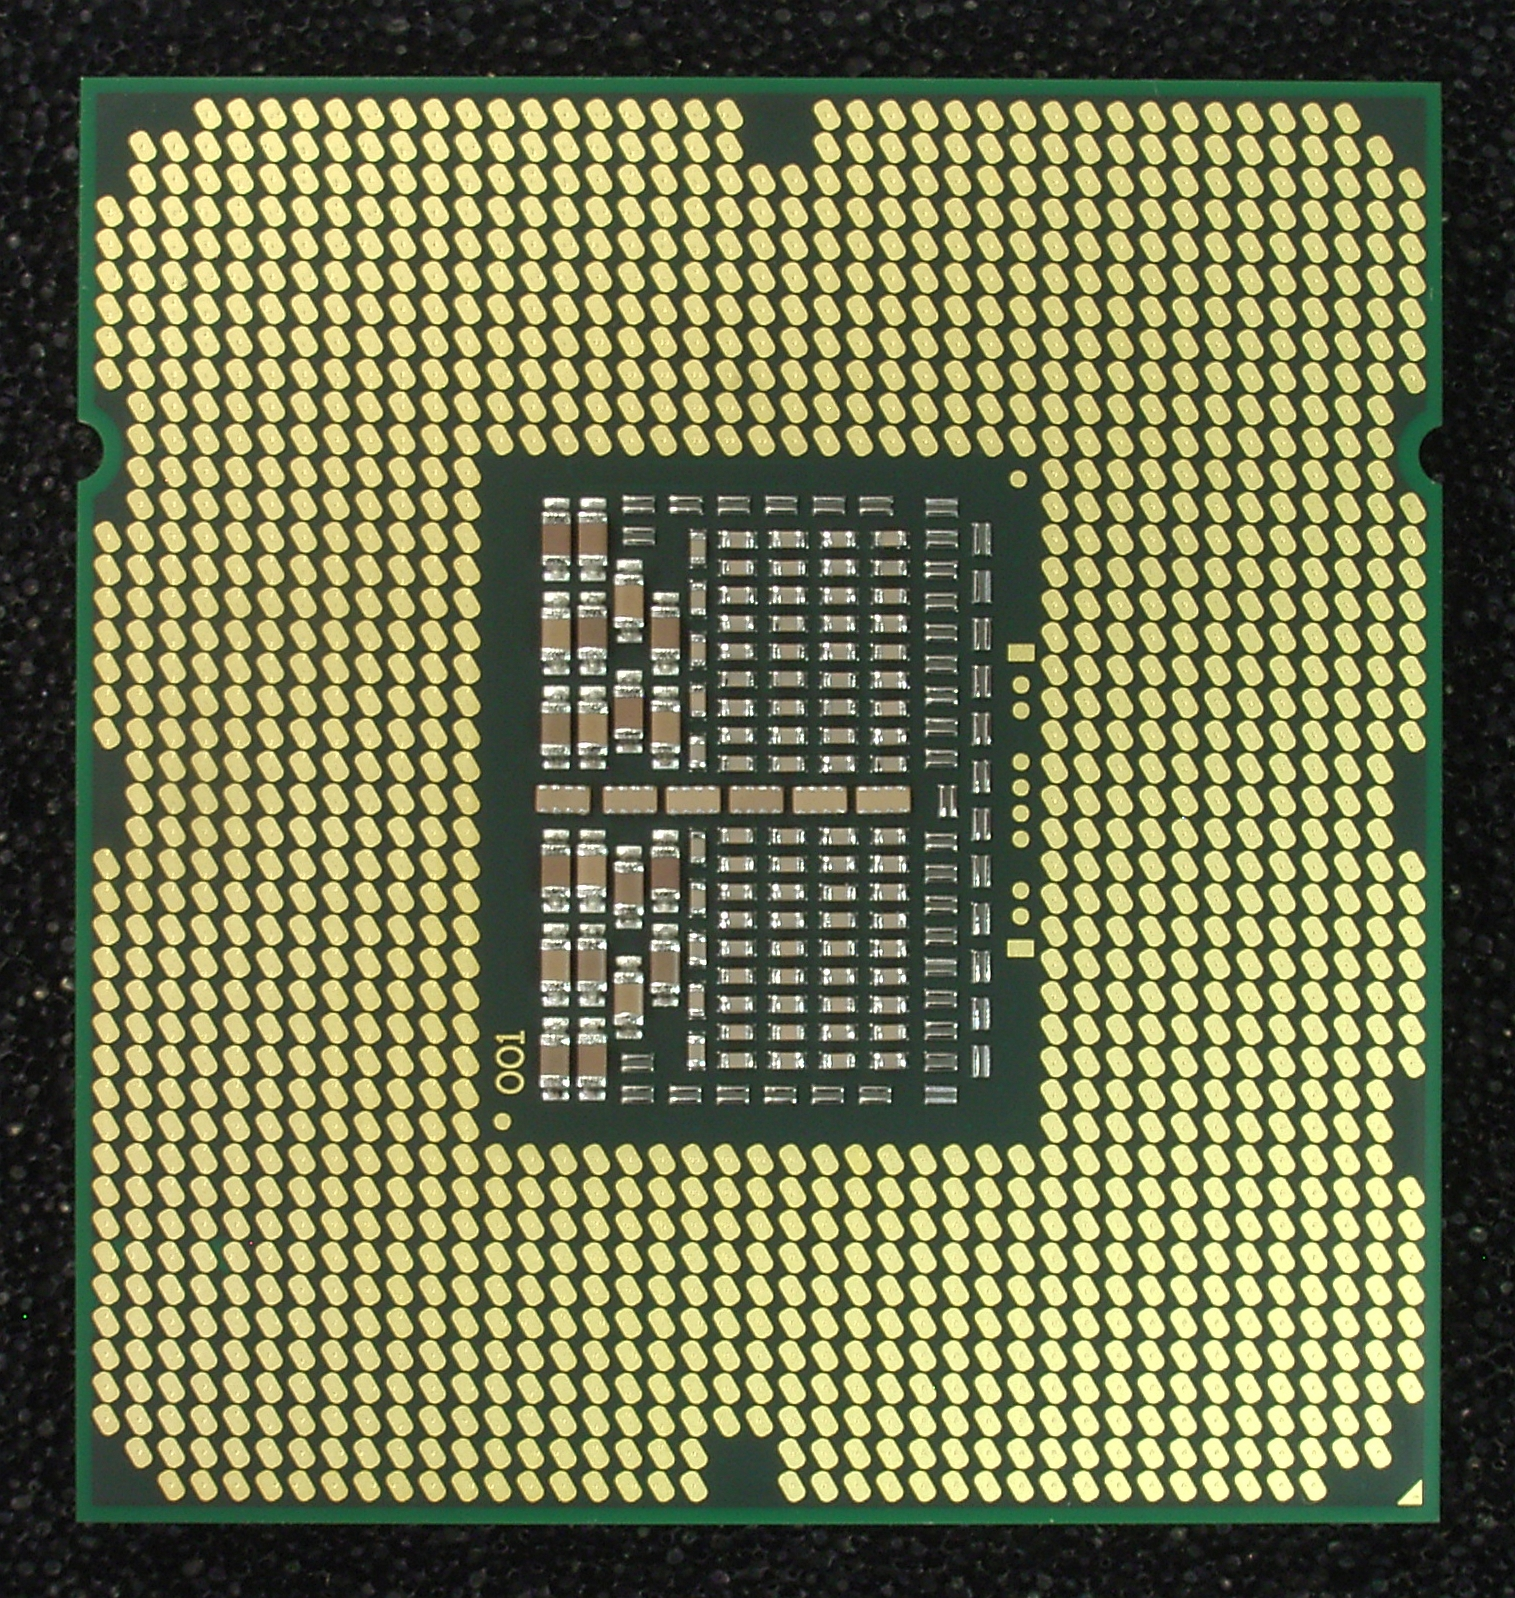
\includegraphics[width=0.3\linewidth]{./media/i7} \\
\caption[Intel Core i7]{ Rainer Knäpper, Free Art License (http://artlibre.org/licence/lal/en/), \url{https://commons.wikimedia.org/wiki/File:Intel_core_i7-975_bottom_R7309730_wp.jpg}}
\end{figure}

	\begin{itemize}
		\item Das Wort “Prozessor” impliziert, dass etwas verarbeitet wird. In Computern geht es hauptsächlich um die Verarbeitung elektrischer Signale, die typischerweise so behandelt werden, dass sie einen der Binärwerte 1 oder 0 haben.
		\item Häufig werden der Begriff “Prozessor” und die Abkürzung CPU (Central Processing Unit) synonym gebraucht, was technisch nicht korrekt ist. Moderne Computer haben neben einer CPU oft auch weitere, aufgabenspezifische Prozessoren:\\
		--  FPU (Floating Point Unit)\\
		-- GPU (Graphical Processing Unit)\\
		-- TPU (Tensor Porcessing Unit) von Google eigens entwickelt für TensorFlow
		\item Die CPU ist also ein Prozessor, aber nicht alle Prozessoren sind CPUs.
	\end{itemize}



Die Kernmarkmale:
\begin{itemize}
	\item \textbf{Befehlssatzarchitektur:}
\begin{itemize}
	\item 	Definiert bestimmte Befehlssätze auf Chip-Ebene, die sogenannten Maschinenbefehle. Dazu gehören zum Beispiel arithmetische, logische oder Transfer-Operationen.
	\item Obwohl Intel und AMD Prozessoren herstellen, die dieselben Anweisungen unterstützen, ist es sinnvoll, nach Anbietern zu unterscheiden, da sie sich herstellerseitig in Bauart, Leistung und Stromverbrauch unterscheiden.
	\item \textbf{Beispiele}
	\begin{itemize}
		\item \link{https://de.wikipedia.org/wiki/X86-Prozessor}{x86-Befehlssatzarchitektur}		\\
		Verweist typischerweise auf die 32-Bit-Befehlssätze der 80386-Nachfolger. nach den Prozessoren der Intel 8086/8080--Reihe benannt.
		\item	x64 (auch x86-64 genannt)\\
		Referenzprozessoren, die sowohl die 32-Bit- als auch die 64-Bit-Anweisungen der x86-Familie unterstützen (rückwärtskompatibel).
		\item	AMD	\\
		Verweist auf die x86-Unterstützung durch AMD-Prozessoren.
		\item	AMD64, Intel64	\\
		Verweist auf die x64-Unterstützung durch AMD-(Intel-)Prozessoren.
	\end{itemize}
\end{itemize}
	\item \textbf{Verarbeitungsbreite/Bitgröße (\textit{Bit size}):}\\
	Bei CPUs bezieht sich diese Zahl sowohl auf die native Größe der von ihr verarbeiteten Daten als auch auf die Menge an Speicher, auf die sie zugreifen kann. Die meisten modernen Systeme sind entweder 32-Bit oder 64-Bit. Grob: Die CPU arbeitet in (32) 64Bit-Blöcken.
	\item \textbf{Taktfrequenz (\textit{clock speed}) [MHz/GHz]:}
\begin{itemize}
	\item Sagt aus, wie schnell ein Prozessor Anweisungen verarbeitet. \item Prozessorgeschwindigkeit ist nur einer der Faktoren, die Systemreaktionszeiten, Wartezeiten und den Durchsatz beeinflussen.
	\item Da man bei Standard Office-Nutzugn eines Rechners nur einen Bruchteil der Rechenleistung einer CPU verwendet, lohnt sich eine höhere Taktfrequenz lediglich bei rechenintensiven Anwendungen, welche die CPU auch 100\% auslasten.
\end{itemize}
	\item \textbf{Cache:}
\begin{itemize}
	\item Die Kosten und der Stromverbrauch eines Arbeitsspeichers mit mehreren Gigabyte, auf den mit CPU-Taktgeschwindigkeiten zugegriffen werden kann, sind unerschwinglich.
	\item Der CPU-Cache-Speicher ist auf dem CPU-Chip integriert, um einen schnellen Puffer zwischen CPUs und Arbeitsspeicher bereitzustellen. Der Cache ist in mehrere Schichten unterteilt, die üblicherweise als L1, L2, L3 und sogar L4 bezeichnet werden. In Fall von Cache gilt: Je mehr, desto besser.
\end{itemize}
	\item \textbf{Kerne (\textit{Cores}):}
\begin{itemize}
	\item 	``Kern/Core'' bezieht sich auf eine einzelne CPU. Zusätzlich zum Core, der eine physische CPU darstellt, ermöglicht Hyper-Threading Technology (HTT) einer einzelnen physischen CPU, mehrere Anweisungen gleichzeitig zu verarbeiten, so dass sie praktisch als mehrere physische CPUs fungiert.
	\item Typischerweise werden mehrere physische Kerne als ein einziger physischer Prozessorchip verbaut.
	\item Auch hier: Standard Office-Anwendungen beanspruchen einen einzelnen Kern kaum. Daher bringt es für Standardanwendungen nicht viel weitere unbeschäftigte Kerne hinzufügen.
	\item Mehr Kerne führen nur dann zur Verbesserung des Durchsatzes wenn sie für die Ausführung von Anwendungen, die so geschrieben sind, dass sie mehrere unabhängige Funktionsabläufe aufweisen, wie z.B. Video-Frame-Rendering, Webseiten-Rendering oder parallele numerische Verfahren (HPC: High Performance Computing) mit mehreren Benutzern.
\end{itemize}
\end{itemize}
\demo{~\\
	Unter Linux:\\~\\
	Die Datei $$\texttt{/proc/cpuinfo}$$ enthält detaillierte Informationen über den oder die Prozessoren eines Systems. Leider sind diese Details nicht allgemeinverständlich. Ein übersichtlicheres Ergebnis liefert der Befehl $$\texttt{\$ lscpu}.$$
}








%SPEICHER
~\\
	\subsubsection{Speicher}
	\begin{figure}[h!]
		\centering
		~\\
		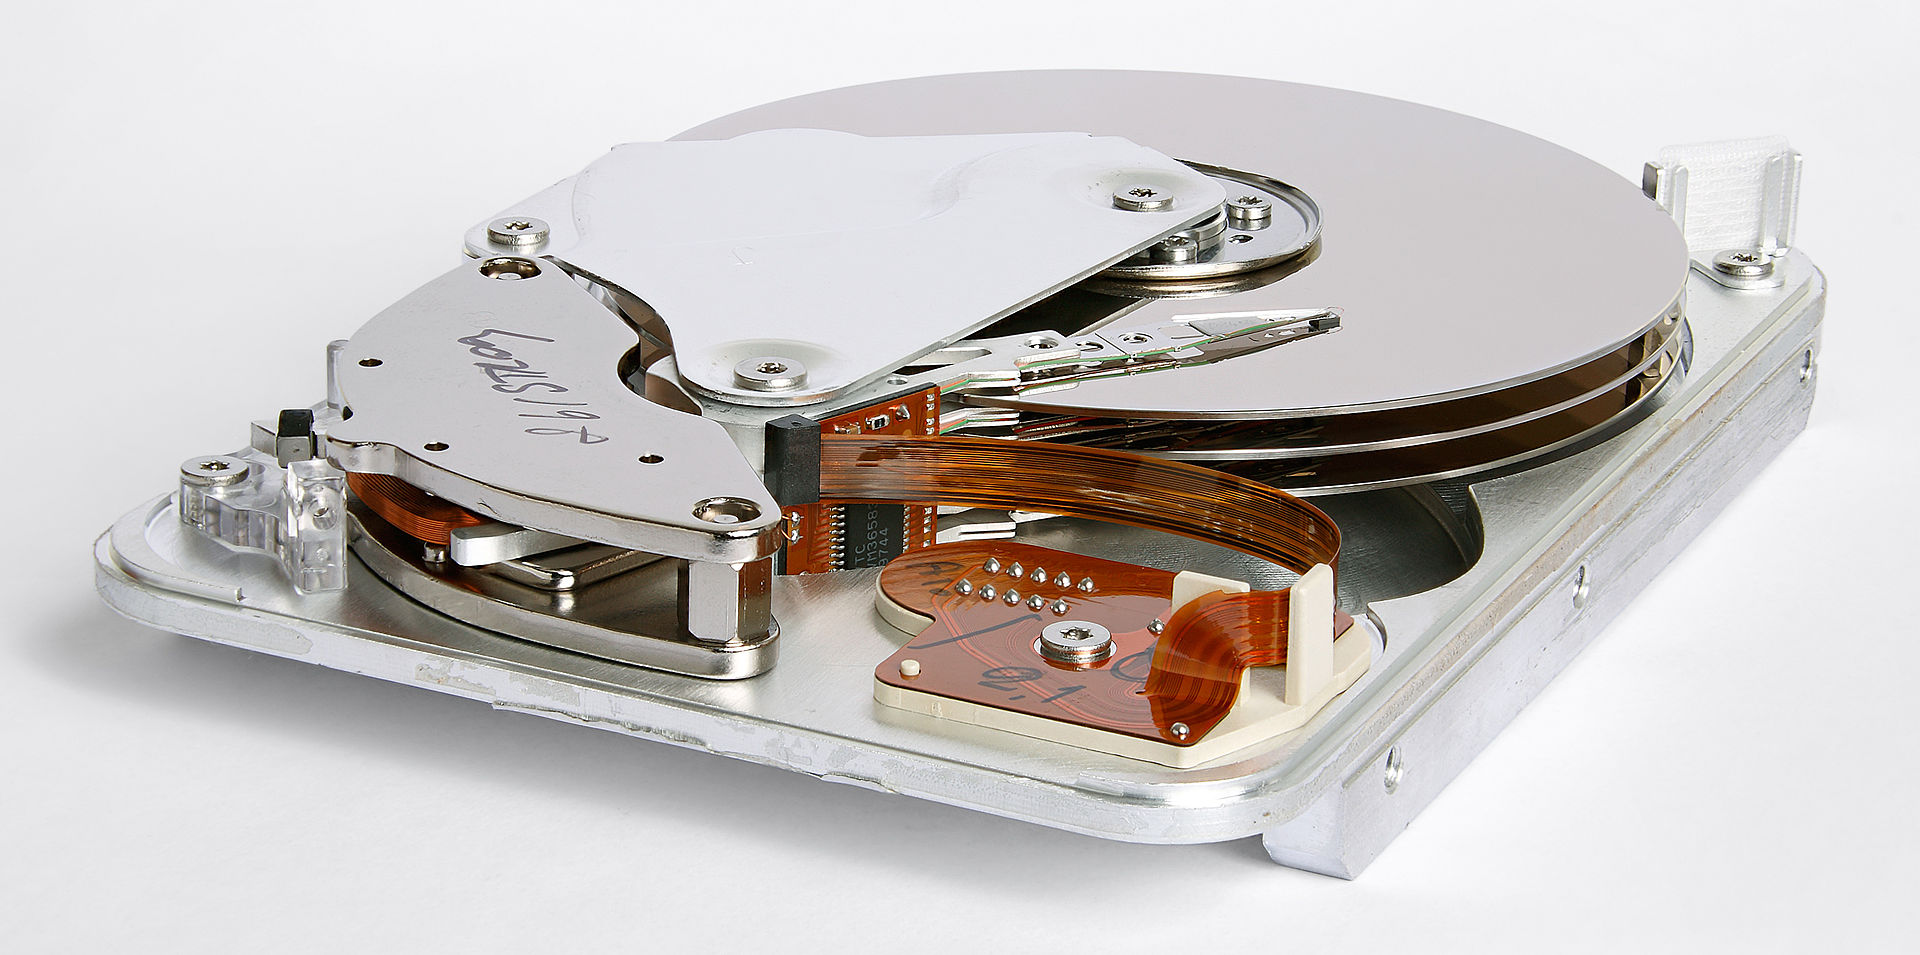
\includegraphics[width=0.5\linewidth]{./media/hdd} \\
		\tiny
		Hard Disk Drive (HDD)\\
		Quelle: Eric Gaba, Wikimedia Commons user, \url{https://de.wikipedia.org/wiki/Festplattenlaufwerk}
	\end{figure}
	\begin{itemize}
		\item Speichergeräte dienen der Aufbewahrung von Programmen und Daten.
		\item Festplattenlaufwerk \textit{Hard Disk Drives} (HDDs) und Halbleiterlaufwerk \textit{Solid State Drives} (SSDs) sind die häufigste Form von Speichergeräten in Servern und Desktops. USB-Speichersticks oder SD-Karten werden selten als primäre Speichermedien verwendet (zu unzuverlässig).
		\item \textbf{HDD} (siehe \link{https://de.wikipedia.org/wiki/Datei:Harddrive-engineerguy.ogv}{Video}):
		\begin{itemize}
			\item  Ein Festplattenlaufwerk speichert Informationen auf einer oder mehreren starren physischen Platten, die mit magnetischen Materialien bedeckt sind, um die Speicherung zu ermöglichen.
			\item Die Platten befinden sich in einem abgedichteten Gehäuse, da Staub oder kleine Partikel die Lese/schreib-Fähigkeit der HDD beeinträchtigen würden.
		\end{itemize}
		\item \textbf{SSD}:\begin{itemize}
			\item  SSDs sind deutlich anspruchsvollere Varianten von USB-Sticks mit wesentlich größerer Kapazität.
			\item Sie speichern Informationen in Mikrochips, so dass es keine beweglichen Bauteile gibt.
		\end{itemize}
	\end{itemize}
\textbf{Vergleichsparameter}
\begin{itemize}
	\item \textit{Kosten}:\\
	SSD bis zu 3-10 mal so teuer pro GB
	\item \textit{Zugriffsgeschwindigkeit} (lesen/schreiben): SSD schneller als HDD, denn\\
	 HDD: Zum Lesen oder Schreiben muss sich eine bestimmte Stelle einer Festplatte an einen bestimmten Ort drehen.\\
	 SSD: Erlauben Direktzugriff.
	\item \textit{Speicherapazität}: 5TB für HDD und 1TB SSD heutzutage üblich\\
\end{itemize}
\textbf{Anschlüsse:}
\begin{itemize}
	\item SCSI (Small Computer System Interface)
	\item SATA (Serial AT Attachment)
	\item USB
\end{itemize}
Diese Interfaces werden typischerweise durch entsprechende Stecker auf der Hauptplatine unterstützt.\\
In den Firmware(UEFI/BIOS)-Einstellungen (Bootmenü) können wir die Reihenfolge festlegen, in der beim ersten Laden auf die Geräte zugegriffen wird (wie oben erwähnt: Notwendig, wenn man von einem anderem Speichermedium booten möchte.)
~\\
%\textbf{RAID}\\
%Speichersysteme, die als RAID (Redundant Array of Independent Disks) bezeichnet werden, sind eine gängige Implementierung zur Vermeidung von Datenverlust. Ein RAID-Array besteht aus mehreren physischen Geräten, die doppelte Kopien von Informationen enthalten.

\demo{~\\Speichergeräte lesen und schreiben üblicherweise Daten in Blöcken von Bytes; man spricht daher auch von \textbf{BLockgeräten}.
~\\~\\
Unter Linux:\\~\\
Mit dem Befehl $$\texttt{\$ lsblk~~~\# ''list block devices''}$$ können Sie die einem System zur Verfügung stehenden Blockdevices auflisten.\\
%~\\`
%\textbf{Gerätedateien} liegen im Verzeichnis /dev und identifizieren physische Geräte, Gerätezugriff und unterstützte Treiber. In modernen Systemen, die SCSI- oder SATA-basierte Speichergeräte verwenden, beginnt der Dateiname der Spezifikation üblicherweise mit dem Präfix sd, gefolgt von einem Buchstaben wie a oder b, der auf ein physisches Gerät verweist. Nach dem Präfix und der Gerätekennung kommt eine Nummer, die eine Partition in dem physischen Gerät angibt. /dev/sda würde also auf das gesamte erste Speichermedium verweisen, während /dev/sda3 die Partition 3 im ersten Speicher bezeichnet.
}

~\\
\textbf{Partitionen}
\begin{itemize}
	\item Ein Speichergerät ist praktisch eine lange Folge von Speicherplätzen. Partitionierung ist der Mechanismus, mit dem man diese Folge in mehrere unabhängige Sequenzen zerlegen kann. Jede Partition wird wie ein einzelnes Gerät behandelt.
	\item Vorteile:
	\begin{itemize}
		\item Verwaltung des verfügbaren Speichers oder die Unterstützung mehrerer \textbf{Dateisysteme} (ext4, vFAT, NTFS,...).
		\item Multi-System: Partitionen ermöglichen es, ein einziges Speichergerät zu haben, das unter verschiedenen Betriebssystemen booten kann
	\end{itemize}
	\item \textbf{Formatierung}:\begin{itemize}
		\item  Zwar erkennt das Betriebssystem (wie Linux) die Speichersequenz eines Raw-Device, aber ein Raw-Device kann nicht ``einfach so'' verwendet werden.
	\item Um ein Raw-Device zu nutzen, muss es formatiert, d.h., ein Dateisystem muss auf das Gerät geschrieben werden.
	\item Dann erst ist können Dateioperationen ausgeführt werden.
	\end{itemize}
%	Ohne ein Dateisystem kann ein Gerät nicht für dateibezogene Operationen genutzt werden.
%	\item Vorsicht: Partionen eignen sich nicht für ein fehlertolerantes Design. Wenn das Gerät ausfällt, fallen alle Partitionen aus.
\end{itemize}

%
%PERIPHERIEGERÄTE
	\subsubsection{Peripheriegeräte}
	\begin{itemize}
		\item Ein Computersystem braucht lediglich eine Kombination aus CPU, Arbeitsspeicher und Speicher. \\
		$\rightarrow$ Aber diese grundlegenden Komponenten interagieren nicht direkt mit der Außenwelt.\\
		$\rightarrow$ Peripheriegeräte sind die Geräte, die den Systemen Input, Output und Zugriff auf den Rest der realen Welt ermöglichen.
		\item Beispiele: Tastatur, Maus, Sound, Video und Netzwerk
%		\item Anschlüsse:\\
%		-- Ethernet-Anschluss zur Unterstützung von Netzwerken\\
%		-- HDMI-Anschluss zur Unterstützung grundlegender grafischer Anforderungen\\
%		-- USB-Anschlüsse (Universal Serial Bus) für die meisten anderen Alltagsgeräte
%		\item Einige Systeme enthalten Peripheriegeräte. Laptops ähneln Workstations, verfügen aber über standardmäßige Anzeige-, Tastatur- und Mausperipheriegeräte.
	\end{itemize}

~\\~\\
\subsubsection{(Geräte-)Treiber}
Wenn eine CPU mit den Endgeräten (z.B. den Laufwerken, Drucker,...) verschiedenster Hersteller zusammenarbeiten soll, dann muss man sich zunächst auf eine gemeinsame Schnittstelle verständigen: Eine Konvention, die eine Verbindung verschiedener Bauteile festlegt.\\
~\\
\textbf{Beispielproblem:}
\begin{itemize}
	\item Ein Textverarbeitungsprogramm kann nicht im Voraus alle verschiedenen Drucker kennen, die
es  einmal bedienen soll.
\item Wenn der Benutzer den Befehl ``Drucken'' auswählt, soll der Druck funktionieren, egal welcher Drucker angeschlossen ist.
\item Dazu bedient sich das Programm einer Schnittstelle, die im Betriebssystem definiert wird; genauer installiert man ein Programm (Treiber), das der Druckerhersteller für das entsprechende Betriebssystem mitliefert und welches die Druckbefehle in Signale für den Drucker umsetzt.
%\item Siehe auch: \textbf{Common Unix Printing System (CUPS)}
\end{itemize}
~\\
\textbf{Allgemein}
\begin{itemize}
	\item  Gerätetreiber (\textit{Device Driver }oder kurz \textit{Driver}) akzeptieren einen Standardsatz von Anfragen und übersetzen diese dann in die entsprechenden Steuerungsaktivitäten des Geräts.
\item Ein Treiber ermöglicht einem Anwendungsprogramm die Benutzung einer
Komponente, \textbf{ohne} deren detaillierten Aufbau zu kennen.
\item Die Anforderungen eines
Anwendungsprogramms an das zugehörige Gerät werden dann vom Betriebssystem an den entsprechenden Treiber umgeleitet, dieser wiederum sorgt für die korrekte Ansteuerung des
Druckers.
\end{itemize}
%
\begin{figure}[h!]
	\centering
	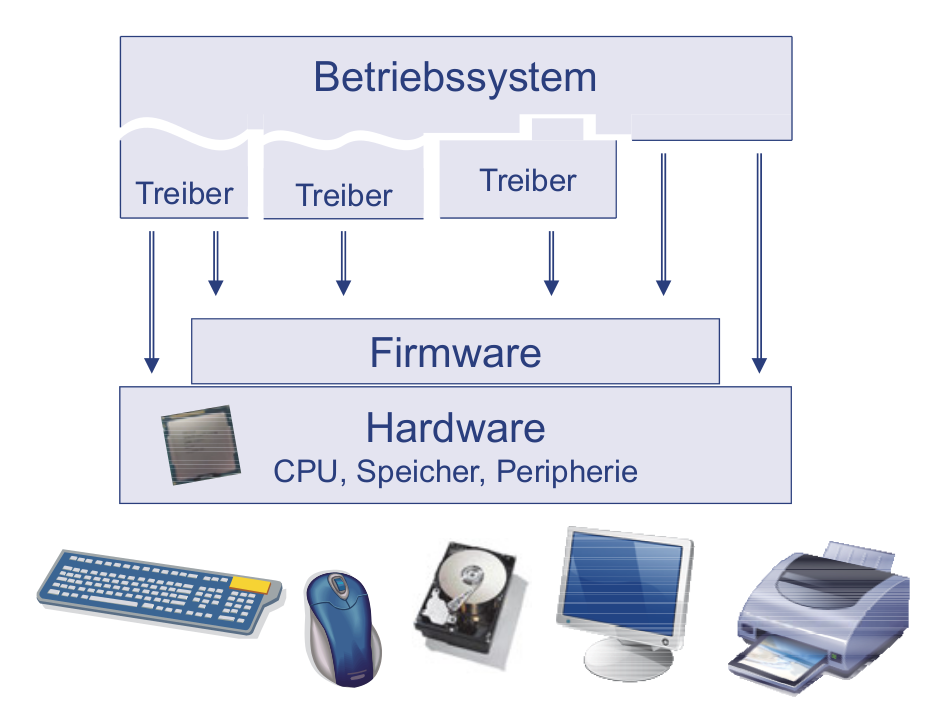
\includegraphics[width=0.5\linewidth]{./media/treiber}
	\caption[Treiber]{Hardware, Treiber und Betriebsystem; Quelle: \cite[Abb. 1.27]{gumm1}}
	\label{fig:treiber}
\end{figure}

%
~\\
\textbf{Anderes Beispiel:} Temperatur- und Luftdrucksensor für einen Raspberry Pi. Der Betriebssystemkernel braucht entsprechende Kerneltreiber, um diesen auszulesen und die Daten dem Benutzer über eine geeignete Schnittstelle zur Verfügung zu stellen (zum Beispiel Textdateien in einem designierten Verzeichnis, das ausgelesen werden kann, um dann in Python damit zu arbeiten).
%
%

% TASKS
\demo{~\\
	Unter Linux:
	\begin{itemize}
		\item \ttt{\$ lshw -short}
		\item \ttt{\$ lscpu}
		\item \ttt{\$ hwinfo ----short}
		\item Für weitere Befehle unter Linux zur Ermittlung von Hardware Informationen siehe zum Beispiel: \url{https://www.binarytides.com/linux-commands-hardware-info/}
\end{itemize}}
\homework{\textbf{Hausaufgaben}
	\begin{enumerate}
		\item Welche Firmware (UEFI oder BIOS) wird auf Ihrem System verwendet?
		\item Wo liegt der Bootloader?
		\item Finden Sie heraus, welcher Prozessor in Ihrem Rechner verbaut ist. Um welche Architektur handelt es sich?
		\item Wie viel GB Arbeitsspeicher (RAM) hat Ihr Rechner?
		\item Welche Festplatten sind eingehangen?
	\end{enumerate}
}

\newpage
\subsection{Betriebssysteme}
\textit{\small(siehe auch \cite[Kap. 2]{gumm2}, \cite[Kap. 6 ]{gumm3})}\\~\\
Zugeschnitten auf die vorhandene Prozessor-Architektur werden Betriebssysteme (genauer Betriebsystemkerne) entwickelt, die Hardware-Ressourcen des Rechners (Speicher, Prozessorleistung, externe Geräte) dem Benutzer zur Verfügung stellen; siehe auch Abb. \ref{fig:betriebssystem}.
Ein Betriebssystem ist damit letztlich ein Programm, das dem Benutzer (\textit{user}) und den Anwendungsprogrammen (\textit{app}) grundlegende Dienste bereitstellt. Diese Dienste  machen das aus, was der Rechner in den Augen eines Nutzers kann.\\
\begin{figure}[h!]
	\centering
	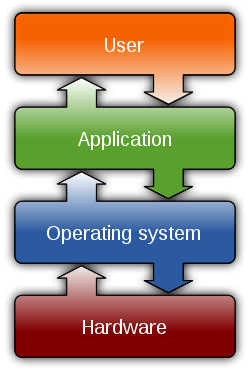
\includegraphics[width=0.2\linewidth]{./media/wiki_os}
	\caption{Quelle: \url{https://de.wikipedia.org/wiki/Betriebssystem}}
	\label{fig:wikios}
\end{figure}
~\\
\textbf{Beispiele}\\
Die meisten Rechner werden zusammen mit einem bereits vorinstallierten Betriebssystem verkauft.
\begin{itemize}
	\item Auf PCs dominiert immer noch \textbf{Microsoft Windows} (aktuell (2022) mit Version Windows 11)
	\item Gefolgt von \textbf{macOS} (exklusiv auf den Rechnern der Firma Apple).
	\item \textbf{Linux} (ein freies, quelloffenes Betriebssystem) dominiert auf Servern und im wissenschaftlichen Bereich.
	\item Auf kleineren Rechnern (Netbooks, Tablets oder Smartphones) ist das auf Linux basierende \textbf{Android} der Firma Google sehr beliebt.
\end{itemize}
Wir werden uns die folgenden Komponenten eines Betriebssystem näher anschauen und anhand von Linux praktisch kennenlernen:
\begin{itemize}
	\item \textbf{Betriebssystemkern}
	\item \textbf{Dateisystem}
	\item \textbf{Mensch-Computer-Schnittstelle:}
	\begin{itemize}
		\item CLI: \textbf{Kommandointerpreter} (Shell)
		\item optionale GUI: \textbf{Desktopumgebung} (inkl. Dateimanager)
	\end{itemize}
\end{itemize}

\demo{\begin{itemize}
		\item 		Der Dateiname eines Betriebssystem-Images beinhaltet häufig Information über die vorgesehene Prozessorarchitektur: z.B. $$\texttt{ubuntu-20.04.2.0-dektop-amd64.iso}.$$
		~\\\url{https://ubuntu.com/\#download}
 \end{itemize}}




\subsubsection{Betriebssystemkern (\textit{kernel})}
Ein \link{https://en.wikipedia.org/wiki/Kernel\_(operating\_system)}{Betriebssystemkern}, auch \textbf{Kernel} genannt, ist der zentrale Bestandteil eines Betriebssystems, auf dem alle weiteren Softwarebestandteile des Betriebssystems aufbauen. Er bildet somit die unterste Softwareschicht des Betriebssystems und hat direkten Zugriff auf die Hardware.
\begin{itemize}
	\item Der Kernel ist in der Regel das erste Programm, dass nach dem Bootloader (siehe oben) gestartet wird.
	\item Er muss mehr Rechte besitzen, um notfalls ein ``abgestürztes'' Programm zu
	beenden, Speicher wieder freizugeben oder den Zugriff auf eine Ressource zu verweigern. Um zu verhindern, dass Benutzerprogramme sich ähnliche Rechte anmaßen,
	muss der Prozessor verschiedene Privilegierungsstufen vorsehen. Die höchste Stufe
	steht nur dem Kern zu.
	\item Er hat völlige Kontrolle über das System.
	\item Befindet sich stets im Speicher (RAM).
\end{itemize}

\demo{\begin{itemize}
		\item Um herauszufinden welcher Linux-Kernel verwendet wird: $$\texttt{\$ uname -r   \#(kernel release)}$$
		oder
		$$\texttt{\$ uname -a   \#(all)}$$
		Output:\\
		5 : Kernel version\\
		8 : Major revision\\
		0 : Minor revision\\
		44 : Patch level\\
		generic : Linux distro/kernel specific additional info
		\item Das GitHub Repository zum Kernel verwaltet vom Linux-Vater Linus Torvalds:
		$$\text{\url{https://github.com/torvalds/linux}}$$
\end{itemize}}

\subsubsection{Dateisysteme (\textit{file system})}
Unter den elementarsten Diensten eines jeden Betriebssystems befinden sich solche, die den
Umgang mit \textbf{Dateien} (engl.: \textit{files}) (=Folge von Bytes) organisieren.
\begin{itemize}
	\item Dateien müssen erzeugt, verändert,
	abgespeichert, umbenannt und gelöscht werden
	\item In die Fülle der existierenden Dateien muss eine Ordnung gebracht werden
	\item Rechte: Der Zugang zu ihnen muss den anderen
	Benutzern des Rechners ermöglicht oder blockiert werden
\end{itemize}
%Für einen Benutzer ist es einfacher und intuitiver, seine Daten (=Folge von Bits) in \textbf{Dateien} (engl. \textit{files}) (=Folge von Bytes) zu organisieren.
Das Betriebssystem muss eine Übersetzung zwischen den von der Hardware angebotenen Blöcken von Bytes und den vom Benutzer gewünschten Dateien gewährleisten. Dazu verwendet es ein \textbf{Dateisystem}.
~\\
Dateien können zu einem \textbf{Verzeichnis} (engl. \textbf{directory}) zusammengefasst werden. Darin findet sich für jede Datei ein Eintrag mit kennzeichnenden Informationen (\textbf{Attribute} genannt) wie:
\begin{itemize}
	\item Dateiname (ggf. auch die „Erweiterung“ ),
\item Dateityp (Normaldatei, ausführbare Datei, Katalogdatei)
\item Länge in Bytes,
\item zugehörige Blöcke (meist reicht ein Verweis auf den ersten Block),
\item Zugriffsrechte (Besitzer, ggf. Passwort, wer hat Lese- oder Schreibrechte)
\item Datum (Erstellung, Änderung, evtl. Verfallsdatum).
\end{itemize}
\demo{
	\begin{itemize}
	\item Partitionen nochmal anschauen, Dateisystem?
		$$\texttt{\$ lsblk -f ~~~\# ( | grep sd)} $$
		(''-f'': Output  info about filesystems.)
\end{itemize}
}






\subsubsection{Schnittstelle zwischen Mensch und Betriebssystem: CLI VS GUI}
Wir klären zunächst folgende Begrifflichkeiten:
\begin{itemize}
	\item \textbf{CLI:} \textit{Command Line Interface} \\
Eine Kommandozeilen-Schnittstelle (\textit{command-line interface}) (CLI)  bezeichnet die Verwendung von Kommandozeilen (Textzeilen) für die Interaktion mit einem Benutzer. Das Programm, welches diese Schnittstelle verwaltet nennt man \textbf{Kommandozeileninterpreter} (z.B. Shell für Betriebssysteme).
%
\item \textbf{GUI:} \textit{Graphical User Interface}\\
Grafische Benutzeroberfläche oder auch grafische Benutzerschnittstelle bezeichnet eine Benutzerschnittstelle mittels grafischer Symbole und Steuerelemente (Widgets). Dies geschieht
\begin{itemize}
	\item bei Computern: mittels einer Maus als Steuergerät,
	\item bei Smartphones, Tablets und Kiosksystemen:  durch Berührung eines Sensorbildschirms.
\end{itemize}
\end{itemize}

\subsubsection*{CLI: Shell}
Als \textbf{Shell} wird der Kommandozeileninterpreter bezeichnet, mittels dessen ein Benutzer über Kommandozeilen mit einem Betriebssystem interagiert. Die Shell (englisch für „Schale“ oder „Hülle“) ist anschaulich die Außenschicht des Betriebssystemkerns.
\begin{itemize}
	\item Kommandozeilen waren historisch die ersten Methoden zur Interaktion mit Betriebssystemen und benötigen lediglich den Textmodus.
	\item Kommandozeileninterpreter sind bei modernen Betriebssystemen auch im Grafikmodus verfügbar, etwa als Terminalemulation (siehe unten).
%Ein Kommandozeilenprogramm läuft somit typischerweise mit den gegebenen Parametern einmal ab, bevor eine erneute Befehlseingabe möglich ist. Ein automatisiertes Abarbeiten mehrerer Kommandos wird auf Unix-artigen Betriebssystemen als Shell-Script bezeichnet.
\end{itemize}

\subsubsection*{GUI: Desktop-Umgebung}
Heute starten die meisten Betriebssysteme unmittelbar mit einer \link{https://en.wikipedia.org/wiki/Graphical_user_interface}{grafischen \textbf{Benutzeroberfläche}} (\textbf{GUI:} Graphical User Interface), der sogenannten \link{https://de.wikipedia.org/wiki/Desktop-Umgebung}{\textbf{Desktopumgebung}}; die technische Umsetzung der sogennanten \textbf{Schreibtischmetapher}\footnote{Die Idee der graphischen Benutzeroberfläche und des Desktops entstand in den 1970er bei Xerox im Palo Alto Research Center (Xerox PARC). Das Konzept von Xerox wurde von der damals noch kleinen Firma Apple übernommen. Nach einem anfänglichen Misserfolg mit dem System Apple Lisa trat der Macintosh seit den frühen 80er Jahren seinen Erfolgszug an.}:
\begin{itemize}
	\item Der Rechner präsentiert grafisch einen Schreibtisch (desktop), auf dem Akten und Ordner (Dateien und Verzeichnisse) herumliegen. Diese Akten können geöffnet und verändert (edit), kopiert (copy) oder in einen Papierkorb geworfen werden (delete).
	\item Man kann die Objekte des Schreibtisches anfassen, verschieben oder aus Ordnern neue Akten herausholen.
\end{itemize}
\begin{itemize}
	\item Erst den grafischen Betriebssystemoberflächen ist es zu verdanken, dass heute
	jeder einen Rechner irgendwie bedienen kann!% und dass es auch leicht ist, mit einem 	bisher unbekannten Programm zu arbeiten, ohne vorher dicke Handbücher zu wälzen.
	\item 	Genau genommen handelt es sich bei den grafischen Oberflächen um Betriebssystemaufsätze\\
	$\to$ Es gibt Betriebsysteme meist in einer desktop und server version (mit oder ohne Desktop-Umgebung; siehe zB \url{https://ubuntu.com/\#download})
%	$\to$ Kann  bei unixoiden Systemen vom Benutzer frei ausgewählt werden (nicht vom Hersteller des Betriebssystems vorgegeben – wie bei Windows oder macOS)
	\item Beispiel GNOME (GNU Network Object Model Environment) 3.36 ist Standard bei Ubuntu 20.04
\end{itemize}
%
~\\
\textbf{Terminalemulator: ``Shell in der GUI''}\\
Eine Terminalemulation\footnote{Als \link{https://de.wikipedia.org/wiki/Emulator}{Emulator} (von lateinisch aemulari, „nachahmen“) wird in der Computertechnik ein System bezeichnet, das ein anderes in bestimmten Teilaspekten nachbildet.} ist ein Computerprogramm, das die Funktion einer Shell innerhalb einer Desktopumgebung grafisch nachbildet, also ein Vermittler zwischen einer Textanwendung und einer grafischen Oberfläche.
%
\demo{
	~\\
	Beispiel UNIX: \textbf{Gnome Terminal} (A terminal emulator for the GNOME desktop)
	\begin{itemize}
		\item Gnome Terminal
\end{itemize}}
~\\
\link{https://en.wikipedia.org/wiki/File_manager}{\textbf{(Navigatorische) Dateimanager (\textit{file manager or browser})} }\\
Ein Dateimanager (englisch File Manager) ist ein Computerprogramm zum Verwalten von Inhalten auf Dateisystemen, die sich auf unterschiedlichen Speichermedien befinden können. Navigatorische Dateimanager stellen die Inhalte eines beliebigen Verzeichnisses umschaltbar in einem Fenster dar.\\
 ~\\
\textbf{Aufgaben:}
\begin{itemize}
	\item übersichtliche Darstellung in Form einer (oft grafischen) Benutzerschnittstelle
	\item Navigation (über Buttons; ähnlich wie im Webbrowser)
	\item Auflisten, das Umbenennen und Verschieben, das Kopieren und das Löschen von Dateien und Verzeichnissen zu den Grundfunktionen
	\item Bearbeitung von Metadaten unterstützter Dateisysteme, wie beispielsweise Dateiattribute, Dateiberechtigungen und Verknüpfung
	\item Netzwerkverbindungen via protocols, such as FTP, HTTP, NFS, SMB or WebDAV. How? browse for a file server (connecting and accessing the server's file system like a local file system) or by providing its own full client implementations for file server protocols.
\end{itemize}
\textbf{Bekannte Beispiele:} %(siehe auch Abb. \ref{fig:filesystem})
\begin{itemize}
	\item \textbf{Nautilus} ist ein freier \textbf{Dateimanager} für unixoide Systeme. Standard-Dateimanager der Desktop-Umgebung \textbf{Gnome}.	Der Quelltext ist gemäß der GNU General Public License (GPL) frei verfügbar.
	\item Der \textbf{Windows-Explorer} (\url{https://en.wikipedia.org/wiki/File_Explorer}) bildet den voreingestellten Dateimanager in der Windows-Betriebssystemsfamilie seit Windows 95.
	\item Der \textbf{apple Finder} ist der Standard-Dateimanager des aktuellen Apple-Betriebssystems macOS (OS X, Mac OS X; ab 2001) und des klassischen Mac OS (1984–2001).
\end{itemize}
\demo{\begin{itemize}
		\item Features anhand von Nautilus demonstrieren.
\end{itemize}}
\homework{\textbf{Hausaufgaben}
	\begin{enumerate}
		\item Welches Betriebssystem verwenden Sie? Welche Version? Wie viel kostet eine Lizenz für Ihr aktuelles Betriebssystem?
	    \item Welches Dateisystem befindet sich auf Ihren Partitionen?
	    \item Welche Desktopumgebung benutzen Sie?
		\item Welchen Dateimanager benutzen Sie und wie können Sie darin die Attribute einer Datei abrufen?
		\item Rufen Sie die Shell (bzw. dessen Emulation als Terminal) Ihres Betriebssystems auf:
	\begin{itemize}
		\item Linux: \ttt{Strg+Alt+T}
		\item \link{https://de.wikipedia.org/wiki/Cmd.exe}{Windows Shell cmd.exe}
		\item \link{https://en.wikipedia.org/wiki/Terminal_(macOS)}{macOS Terminal.app}
	\end{itemize}
	\end{enumerate}
}
%%%%%%%%%%%%%%%%%%%%%%%
% FREE SOFTWARE
%%%%%%%%%%%%%%%%%%%
%{\color{gray}
%\subsection{Begriffsklärung: Non-Free Software, Free Software, Open-Source, Freeware}
%\subsubsection{1970er/80er Unfreie Software (proprietär)}
%Proprietary software, also known as non-free software,~\\
%Proprietäre Software bezeichnet eine Software, die das Recht und die Möglichkeiten der Wieder- und Weiterverwendung sowie Änderung und Anpassung durch Nutzer und Dritte stark einschränkt. Ursprünglich war dies durch eine Abhängigkeit der Software von der Hardware bedingt. Die Praxis, Quelltexte von Computerprogrammen unter Verschluss und damit im engeren Sinne „proprietär“ zu halten, kam mit der zunehmenden öffentlichen Verbreitung von Computern mit gleichen Mikroprozessoren in den frühen 1980er Jahren auf.[1] Es gibt zahlreiche Mechanismen, die eine Software „proprietär“ machen und halten können: durch Softwarepatente, das Urheberrecht, Lizenzbedingungen (EULAs), das Aufbauen der Software auf herstellerspezifischen, nicht veröffentlichten Standards und die Behandlung des Quelltextes als Betriebsgeheimnis (englisch closed source)
%Sind eine oder mehrere Bedingungen der von der FSF aufgelisteten Freiheiten nicht erfüllt, wird die Software als proprietär oder „unfrei“ (im Sinne fehlender Freiheiten) bezeichnet.
%\subsubsection{1980er: Freie Software (FSF) und GNU}
%~\\
%die Freiheit der Kontrolle über die Software (und zwar uneingeschränkte Freiheit der Kontrolle und Unabhängigkeit durch Erhalt des genauen Quellcodes, um Analysen und Änderungen der Software zu erlauben[Anm. 2]),
%die soziale Freiheit der Kollaboration, um aktiv mit beliebigen anderen Nutzern und Entwicklern kooperieren zu können (die Software darf kopiert und weitergegeben werden,[Anm. 3] im Original oder mit Veränderung).
%~\\
%Um dem GNU-Projekt einen logistischen, juristischen und finanziellen Rahmen zu geben, gründete Stallman 1985 die gemeinnützige \textit{Free Software Foundation} (FSF).~\\
%Der ältere Begriff Freie Software wird bereits seit den 1980ern von der Free Software Foundation (FSF) verwendet. Eine Fehlassoziation von Freier Software mit Freeware war häufig, da im Englischen frei für kostenlos wie auch Freiheit stehen kann[16] und außerdem freie Software in den meisten Fällen wirklich auch kostenlos erhältlich ist. Da mit Frei aber wirklich nur Freiheit von der FSF gemeint war, prägte diese den Slogan, „free speech, not free beer“ – „freie Meinungsäußerung, nicht Freibier“, um einer Assoziation von Freier Software mit kostenloser Software entgegenzuwirken.
%
%Zitat: “The word ‘free’ in our name does not refer to price; it refers to freedom.
%
%First the freedom to copy a program and redistribute it to your neighbors, so that they can use it as well as you.
%Second, the freedom to change a program, so that you can control it instead of it controlling you; for this, the source code must be made available to you.”
%~\\~\\
%Das GNU-Projekt entwickelt das Betriebssystem GNU, das von Richard Stallman mit dem Ziel gegründet wurde, ein freies, unixähnliches Betriebssystem zu schaffen, das sicherstellt, dass die Endbenutzer die Freiheiten haben, es verwenden, untersuchen, verbreiten (kopieren) und verändern zu dürfen. Software, deren Lizenz diese Freiheiten garantiert, wird Freie Software (engl. Free Software) genannt, GNU ist in diesem Sinne frei.\\~\\
%Die \textbf{GNU General Public License }(kurz GNU GPL oder GPL; aus dem Englischen wörtlich für allgemeine Veröffentlichungserlaubnis oder -genehmigung) ist die am weitesten verbreitete Softwarelizenz, die einem gewährt, die Software auszuführen, zu studieren, zu ändern und zu verbreiten (kopieren). Software, die diese Freiheitsrechte gewährt, wird Freie Software genannt; Die GNU GPL wurde im Januar 1989 von Richard Stallman, dem Gründer des GNU-Projekts, geschrieben.
%\subsubsection{1990er: Open Source (OSI)}
%Der Begriff Open Source (zu deutsch „quelloffen“) wurde 1998 von den Gründern der Open Source Initiative (OSI) eingeführt: Eric S. Raymond, Bruce Perens und Tim O’Reilly. Sie wollten den pragmatischeren Ansatz derartiger Software in den Mittelpunkt stellen, statt auf eine (aus ihrer Sicht) möglicherweise abschreckend wirkende, moralisch aufgeladene und polarisierende Freie-Software-Idee zu setzen.[15][16] Quelloffene Software wird von ihnen als vorteilhaftes Entwicklungsmodell beschrieben, wobei die Frage, ob Software quelloffen sein sollte, dort eine rein praktische und keine ethische Frage ist.
%Als Open Source (aus englisch open source, wörtlich offene Quelle) wird Software bezeichnet, deren Quelltext öffentlich und von Dritten eingesehen, geändert und genutzt werden kann. Open-Source-Software kann meistens kostenlos genutzt werden.
% Der Begriff Open Source assoziiert die Verfügbarkeit des Quelltextes, sagt aber nichts über die gewährten Verwendungsrechte und Nutzungsfreiheiten aus
% Die Open Source Initiative (OSI) wendet den Begriff Open Source auf all die Software an, deren Lizenzverträge den folgenden drei charakteristischen Merkmalen entsprechen und die zehn Punkte der Open Source Definition erfüllen:
%\subsubsection{Freeware}
%Free-Beer-Verkauf beim Isummit 2008 illustriert Free as in Freedom, not free as in free beer: Rezept und Label des Biers sind unter der CC-BY-SA, also frei wie in Freiheit, es ist aber nicht kostenlos wie Freibier, da es für 500 Yen verkauft wird.[14]
%→ Hauptartikel: Freeware
%
%Das englische Wort free hat zwei unterschiedliche Bedeutungen und steht in dem seit 1982 gebräuchlichen Begriff Freeware für „kostenfrei“ (genauer für „kostenlose Software“); in Freie Software (englisch Free Software) steht es für „Freiheit“ (genauer für „freiheitsgewährende Software“). Englischsprachige Aktivisten machen die Unterscheidung mit free as in free beer („frei wie Freibier“) und Free as in Freedom („frei wie in Freiheit“) deutlich.
%
%Freeware räumt dem Benutzer nicht die von der Free Software Foundation aufgelisteten Freiheiten ein, sondern die der individuellen Lizenzvereinbarung mit dem Urheber. Daher gilt sie als „unfreie“ Software.
%
%Freie Software enthält hingegen die genannten Freiheiten und kann, muss aber nicht kostenlos sein.
%}

%{\color{gray}
%
%\subsection{2.6 X Window System}
%Grafische Benutzeroberflächen haben sich unter UNIX nur langsam durchgesetzt.
%Durch seine Verbreitung im technisch-wissenschaftlichen Bereich und durch seine
%Abwesenheit auf PCs blieb UNIX lange Spezialisten vorbehalten, für die die Beherr-
%schung der UNIX-Kommandosprache keine Schwierigkeiten bedeutete. Die Handha-
%bung mit Maus und Fenstern beschleunigte die Arbeit nicht unbedingt und war so2.6 X Window System
%|
%201
%eher eine Last als eine Erleichterung. Mit UNIX-Kommandos und Befehlstasten in
%Verbindung mit UNIX-Werkzeugen, wie z. B. emacs, kann ein UNIX-Spezialist schnell
%und gezielt umgehen.
%Mit der Schnelligkeit, mit der neue Anwendungen entstehen, wächst jedoch
%der Druck, neue Software auszuprobieren und anzuwenden, ohne vorher Komman-
%dos, Befehlstasten oder überhaupt ein Manual zu studieren. Hierbei ist eine intui-
%tive Benutzeroberfläche von Vorteil. Heute stattet jeder Workstation-Hersteller sein
%Rechner-Betriebssystem daher mit einer grafischen Oberfläche aus. Wären diese Ober-
%flächen nicht kompatibel, dann wäre dies von Nachteil für die Portabilität von UNIX-
%Anwendungen. Andererseits möchte jeder Hersteller seine Oberfläche mit dem spezi-
%ellen look and feel ausstatten, der sie im Vergleich mit dem Konkurrenten hervorhebt.
%Vor diesem Hintergrund wurde 1984 an der US-amerikanischen Universität MIT
%(Massachusetts Institute of Technology) das X-Fenstersystem (X Window System) ent-
%wickelt, dessen Version 11 aus dem Jahre 1987 sich als X11-Standard in der UNIX-Welt
%etabliert hat. X ist ein netzwerkunabhängiges Fenstersystem, das auf den Rechnern
%vieler Hersteller, z. B. auch auf dem x86-PC, läuft. Voraussetzung ist allerdings ein
%grafikfähiger Bildschirm nebst Tastatur und Maus. Eine X-Applikation kann sich auf
%mehrere Rechner in einem Netzwerk verteilen. Diese Rechner spielen dabei verschie-
%dene Rollen:
%– Der X-Display-Server ist Anbieter der Ein- und Ausgabedienste. Er stellt mit seinem
%Bildschirm die Fenster (X-Windows) dar und registriert Maus- und Tastatureinga-
%ben.
%– Ein oder mehrere X-Clients sind die Kunden oder Nutzer der Server-Dienste. Ge-
%mäß dem X-Protokoll fordern sie Ein- und Ausgabedienste von dem Server an. Die
%auf den X-Clients laufenden Programme können beliebige UNIX-Programme sein:
%Datenbanken, Editoren, Compiler etc.
%Typischerweise sind Rechner heute in lokalen und globalen Netzen eingebunden.
%Demgemäß können X-Clients und X-Server auf verschiedenen Rechnern eines Netzes
%ablaufen, andererseits ist es aber auch möglich, dass sowohl Client als auch Server
%auf demselben Rechner zu Hause sind. Das X-System ist damit ein Beispiel für ein in
%der Netzwelt häufig anzutreffendes Konzept der Client-Server-Architektur.
%Was ist damit gewonnen? Angenommen, dass ein Benutzer vom Rechner auf sei-
%nem Schreibtisch eine Datenbankabfrage starten möchte, die ihm Aufschluss über die
%in einer entfernten Bibliothek vorhandenen Buchtitel zu einem bestimmten Thema
%gibt. Das Ergebnis soll in einem Fenster dargestellt werden, in dem man mithilfe einer
%scrollbar die gelieferten Titel in aller Ruhe ansehen kann. Wegen der begrenzten Ka-
%pazität der Netzverbindung, aber auch aus anderen Gründen wäre es unsinnig, wenn
%der entfernte Bibliotheksrechner die Pixel des Rechners auf dem Schreibtisch des Be-
%nutzers zeichnen müsste, seine Mausbewegungen registrieren und darauf reagieren
%sollte. Als X-Client erwartet das Datenbankprogramm von dem X-Server des Benut-
%zers lediglich, dass dieser ein Fenster mit Rollbalken bereitstellt und die gefundenen202 | 2 Betriebssysteme
%Namen darin darstellt. Solange der Betrachter mit Maus und Rollbalken diese Liste
%inspiziert, ist der Bibliotheksrechner nicht involviert. Erst wenn Mausereignisse oder
%Tastatureingaben zu einer weiteren Anfrage führen, führt er den nächsten Befehl aus.
%Insofern ist es ihm auch gleichgültig, in welcher Farbe, Größe oder welchem Stil die
%Fenster des Servers erscheinen, allein die Funktionalität – Fenster mit Rollbalken plus
%Inhalt – ist relevant und wird durch das Netz übertragen.
%In der Tat bietet ein X-Server allein noch keine überwältigende Benutzeroberflä-
%che. Eine Reihe von nützlichen Hilfsmitteln steht aber zur Verfügung, die es gestatten,
%auf dem X-Server eine nützliche Oberfläche zu gestalten. Diese Hilfsmittel sind übli-
%cherweise selber als X-Clients konzipiert. Die wichtigsten Clients sind dabei der so
%genannte Window-Manager, der xterm Terminal-Emulator sowie eine Reihe von nütz-
%lichen Hilfsmitteln, so genannte utilities.
%
%
%\textbf{2.6.1 Window-Manager und Terminal Emulator}
%Der Window-Manager ist ein Client, der es erlaubt, die Größe und die Position von
%Fenstern zu bestimmen und zu verändern. Mit ihm kann man Fenster verschieben,
%überlappen, zu Icons verkleinern, öffnen und beliebig in der Größe verändern. Der
%Window-Manager ist, als Client, selbst ein X-Programm und kann beliebig ersetzt wer-
%den. Ein populärer Window-Manager heißt uwm, für universal window manager, aber
%es gibt eine Reihe von Alternativen wie Sawfish, kwm oder KWin.
%Ein Terminal-Emulator ist ein Fenster, in welchem man ein Terminal nachbilden
%kann. Das Programm xterm etwa emuliert z. B. das früher weitverbreitete DEC VT102-
%Terminal. In dem Terminal-Fenster wird im VT102 Modus jeder Tastendruck so inter-
%pretiert, als wäre er an dem VT102-Terminal geschehen und auch die Ausgabe be-
%schränkt sich auf den Textmodus des VT102. Eine solche Verbindung im Textmodus
%ist oft bei Netzverbindungen nötig, etwa bei einem login auf einem entfernten Rech-
%ner, rlogin, oder bei einer ftp- oder telnet-Verbindung. Da der X-Server eine Reihe von
%Clients gleichzeitig bedienen kann, dürfen mehrere solcher Terminalfenster zur sel-
%ben Zeit geöffnet sein. So kann man zum Beispiel in einem Fenster Text editieren und
%in einem anderen Fenster Dateien transferieren. Wie bei den meisten X-Clients lässt
%sich durch eine Reihe von Optionen das Verhalten von xterm auf vielfältige Weise den
%Benutzerwünschen anpassen.
%
%
%\textbf{2.6.2 Grafische Oberflächen}
%Wenn auch X11 zum Standard für grafikorientierte Programme geworden ist, so spricht
%nichts dagegen, dass Firmen ihren Produkten ein eigenes look-and-feel, also ein cha-
%rakteristisches, abgestimmtes Aussehen geben. Das X Window System stellt eine
%Grundfunktionalität zur Verfügung, auf der firmeneigene Benutzeroberflächen auf-
%setzen können. Diese Benutzeroberflächen können sich durch eine eigene Gestaltung
%der grafischen Elemente oder auch durch besondere Funktionalität auszeichnen.2.7 MS-DOS und MS-Windows
%|
%203
%Damit z. B. alle Anwendungen der Firma SUN in gewisser Weise einheitlich zu be-
%dienen waren, wurde in einer OPEN LOOK genannten Spezifikation eine grafische
%Benutzeroberfläche spezifiziert. An diese Spezifikation sollten sich Entwickler hal-
%ten, damit neue Software sofort intuitiv bedienbar war. Eine Implementierung einer
%Benutzeroberfläche, die sich an die OPEN LOOK-Spezifikation hielt, bot SUN in dem
%OpenWindows-System an.
%OPEN LOOK mit OpenWindows blieb aber beileibe nicht die einzige grafische Be-
%nutzeroberfläche, die auf X11 aufsetzt. Es wurde durch das System OSF/Motif der Open
%Software Foundation abgelöst. Des Weiteren lässt sich auf X11 auch die Benutzerober-
%fläche von MS-Windows oder die des Apple Macintosh aufsetzen.
%OPEN LOOK und Motif wurden schließlich durch das Common Desktop Environ-
%ment (CDE) abgelöst. Ein Ziel war, in Konkurrenz zu Microsoft Windows einen von
%vielen Firmen unterstützen UNIX-Desktop Standard zu schaffen. Ab 1995 waren die
%ersten CDE-Implementierungen verfügbar. Das ursprünglich proprietäre CDE wurde
%später zum Vorbild für die freien Oberflächen KDE und Gnome, die heute in Linux
%Distributionen dominieren.
%
%\subsection{2.7 Windows}
%Als im Jahre 1981 IBM einen Personal Computer (PC) auf den Markt brachte, konn-
%te niemand ahnen, dass ein Jahrzehnt später schon über 50 Millionen PCs verkauft
%sein würden. Mittlerweile sind es höchstwahrscheinlich weit mehr als eine Milliar-
%de geworden. Natürlich hat sich der ursprüngliche PC weiterentwickelt, selbst IBM
%ist aus dem PC Geschäft ausgestiegen und hat dieses an die Firma Lenovo verkauft.
%Der ursprüngliche Prozessortyp 8088 von Intel mit 16-Bit-Registern, aber nur 8 Bit
%breitem Datenbus, wurde nacheinander ersetzt durch die Typen 286, 386, 486, Pen-
%tium, Core Duo und Core i. Die von der Firma AMD entwickelten Athlon-, Phenom- und
%FX-Prozessoren konkurrieren mit den aktuellen Intel Modellen und sind in der Leis-
%tungsfähigkeit durchaus vergleichbar. Die von AMD eigenständig entwickelte 64-Bit
%Erweiterung der x86 Prozessorfamilie war so erfolgreich dass sie von Intel übernom-
%men wurde und mittlerweile in allen neueren x86 Prozessoren zur Verfügung steht.
%Dennoch trägt auch der neueste, ausgereifteste und schnellste PC noch eine Ver-
%pflichtung mit sich, die von seinem Vorfahren stammt: Millionen von Anwendern ha-
%ben viel Geld und Training in Software investiert, was sie nicht aufgeben möchten.
%Was den Prozessor angeht, ist das Problem technisch lösbar. Neue Prozessoren
%werden als Erweiterung der bisherigen Prozessoren konzipiert. Der neue Prozessor
%beherrscht immer noch die Befehle des Vorgängermodells und einige mehr und hat
%noch die gleiche Registerstruktur, deren Breite sich lediglich verdoppelt hat. So wur-
%den im Übergang vom 80286 zum 80386 im Jahre 1986 die Register von 16 Bit zu 32 Bit
%erweitert, auf neueren Rechnern sogar zu 64 Bit. Die neuen 64-Bit-Allzweckregister
%RAX, RBX, RCX und RDX beinhalten nun die vormaligen 32-Bit-Allzweckregister EAX,204 | 2 Betriebssysteme
%EBX, ECX und EDX in den niederwertigen 32 Bit und diese wiederum die ehemaligen
%16-Bit-Allzweckregister AX, BX, CX und DX in den niederwertigen 16 Bit, so dass alte
%Assemblerprogramme weiter verwendbar sind. Zusätzlich besitzen die neuen Prozes-
%soren einen Modus, in dem sie den alten 8088-Prozessor simulieren. Diesen Modus
%nennt man den real mode.
%Nun wäre es von Vorteil, wenn man alte Software im real mode laufen lassen und
%für die neu erworbene Software die neuen Tricks des Prozessors nutzen könnte. Un-
%glücklicherweise ergibt sich aber eine Schwierigkeit: das Betriebssystem MS-DOS. Da
%de facto jedes Benutzerprogramm auf die Dienste des Betriebssystems zurückgreifen
%muss, stellt sich auch hier das Problem der Kompatibilität zu alten Versionen, für die
%die Software vielleicht auch einmal geschrieben und getestet worden ist.
%Hätte man im Jahre 1981 ahnen können, in welche Bereiche der PC einmal vor-
%stoßen und welche Speichergrößen einmal realistisch werden würden, so hätte man
%MSDOS anders konzipiert. Bald wurde dieses Betriebssystem aber das größte Hemm-
%nis in der Ausnutzung der Möglichkeiten des PCs. Bereits der PC/AT von 1984 konnte
%16 MByte Speicher adressieren, die späteren Prozessoren (seit 1986) 4 Gigabytes. MS-
%DOS jedoch konnte bis Ende der 80er Jahre gerade mal ein Megabyte verwalten, so viel
%wie 1981. Nur im so genannten protected mode des Prozessors, der aber inkompatibel
%zu DOS ist, kann auf diesen Speicherbereich zugegriffen werden.
%Die erste Version von MS-DOS wurde 1981 von der Firma Microsoft erstellt. Das
%System war eng an das damals im Home-Computer-Bereich populäre Betriebssys-
%tem CP/M angelehnt. Da auch IBM davon ausging, dass der IBM-PC hauptsächlich
%für Spielprogramme genutzt werden würde, schien dies eine gute Wahl. Da der erste
%IBM-PC 64 kByte Speicher besaß, erschien ein Betriebssystem, das für bis zu 1 MByte
%Hauptspeicher ausgelegt war, mehr als ausreichend auch für künftige Versionen. Die
%Folge war, dass bis zur Einführung von Windows 95 die meisten Benutzer aus Kompa-
%tibilitätsgründen immer noch auf MS-DOS angewiesen waren und von ihren bis zu 16
%MByte installierten Hauptspeichern nur 640 kByte uneingeschränkt für Programme
%nutzen konnten. Zudem betrieben sie den Prozessor im real mode, denn nur in diesem
%Modus lief das Betriebssystem.
%Obwohl MS-DOS technisch lange überholt war, blieb es bis Mitte der 90-er Jahre
%mit Abstand das meistgenutzte Betriebssystem der Welt. Microsoft hatte ihm 1990 eine
%grafische, mit der Maus zu bedienende Oberfläche gegeben. Doch das neue System,
%Windows 3.11, benötigte als Basis immer noch das 1981 konzipierte Betriebssystem
%MS-DOS.
%Das völlig neu entwickelte Windows NT sollte Microsofts Betriebssystem für High-
%End-PCs, Workstations und Server sein. Mit der Version 5.0 änderte Microsoft die Be-
%zeichnung zu Windows 2000. Eine neuere Version wurde ab Herbst 2001 unter dem
%Namen Windows XP angeboten. Dessen Nachfolger erschien als Windows Vista und
%war nie besonders populär im Gegensatz zu den Nachfolge-Versionen Windows 7 und
%Windows 8 sowie dem aktuellen Windows 10.
%
%\textbf{2.7.5 Windows 10}
%Mit Windows 10 wollte Microsoft ein Betriebssystem schaffen, das auf allen Rech-
%nertypen, dazu gehören seit einiger Zeit auch Tablets und Smartphones, gleich aus-
%sieht und gleich zu bedienen ist. Da Windows als Betriebssystem auf Smartphones
%nur einen sehr geringen Marktanteil hat, schien dies eine gute Strategie. Um dies zu
%unterstützen wurde das Betriebssystem bis Sommer 2016 kostenlos verteilt. Neu in
%Windows 10 ist auch der Nachfolger des Internet Explorers, Windows Edge, sowie ei-
%ne Sprachassistentin Cortana ähnlich wie Apple’s Siri und Google Now. Heftig kritisiert
%wurde Microsoft für die Unmenge privater Nutzerdaten, die ständig an Microsoft über-
%tragen werden. Die Möglichkeiten, sich davor zu schützen sind versteckt und werden
%von den Wenigsten wahrgenommen werden. Die Hoffnung von Microsoft, mit Win-
%dows 10 einen größeren Anteil am Markt der Smartphone Betriebssysteme zu sichern,
%wurden enttäuscht, hier dominiert eindeutig Android, gefolgt von Apple’s iOS; Win-
%dows muss sich mit einem fast vernachlässigbaren Marktanteil von weniger als 2 %
%begnügen.
%
%
%\subsection{2.8 Sonstiges zu OS}
%Viele Jahre hatten MS-DOS und der Nachfolger Windows den Markt der Betriebssys-
%teme für x86-PCs beherrscht. Jahrelang mussten die Anwender mit den Mängeln von
%MS-DOS fertig werden. Als dieses Betriebssystem endlich von Windows abgelöst wur-
%de, krankte jenes unter dem Zwang der Abwärtskompatibilität zu DOS. Diese Abwärts-
%kompatibilität war das erfolgreichste Geschäftsprinzip von Microsoft, hatte man da-
%durch doch immer die größte existierende Softwarebasis mit im Boot. Die Abwärts-
%kompatibilität war für jeden Benutzer, auch für den, der nicht mehr an DOS interes-
%siert war, teuer erkauft. Legende ist die Instabilität der frühen Windows-Versionen,
%ihr Ressourcenhunger und ihre Größe. Mit jeder neuen Version wurde ein neuer Rech-
%ner fällig, da für ein vernünftiges Arbeiten der Prozessor zu langsam war, Festplatte
%und Hauptspeicher viel zu klein dimensioniert. Natürlich bot das Betriebssystem im-
%mer mehr Features, wurde immer bequemer zu bedienen und immer leistungsfähiger.
%Aber dennoch ist die Frage berechtigt, ob die stetige Aufblähung des Betriebssystems
%ein notwendiger Preis für die gebotenen Fähigkeiten ist.
%Die Antwort haben am eindrucksvollsten der finnische Student Linus Torvalds
%und mit ihm Tausende von enthusiastischen Idealisten gegeben, die mit Linux (siehe
%S. 166) ein leistungsfähiges, stabiles und ausgereiftes Betriebssystem geschaffen und
%kostenlos zur Verfügung gestellt haben. Linux gewinnt vor allem durch seine Stabili-2.8 Alternative PC-Betriebssysteme |
%209
%tät, aber auch durch die explosionsartig zunehmende Softwarebasis, die von profes-
%sioneller Qualität und dazu noch kostenlos ist, sowohl im privaten als auch im kom-
%merziellen Bereich stetig an Bedeutung.
%Wie klein kann ein grafisches Betriebssystem sein? Ein grafisches Betriebssystem
%benötigt heute mindestens eine grafische Benutzeroberfläche, Unterstützung ver-
%schiedenster Grafikkarten mit unterschiedlichen Auflösungen, Mausunterstützung,
%Modemanschluss, TCP/IP, Netzwerkanbindung und natürlich Grundsoftware wie Da-
%teimanager, Texteditor, einen Browser mit JavaScript-Unterstützung und Plug-Ins für
%verschiedene Bildformate. Selbstverständlich sollte es auch via Plug and Play die
%Hardware-Konfiguration selbstständig erkennen.
%~\\~\\
%Ansonsten wird der Markt der TabletPC sowie der Smartphones von den Betriebs-
%systemen iOS und Android dominiert. iOS wird von Apple auf seinen iPads, iPhones
%und iPods eingesetzt.
%Abb. 2.15. Android Logo
%Android ist eine Neuentwicklung unter Federführung der Firma Google. Es ba-
%siert auf dem Linux Kern und einer Java-Platform. Letzteres ist quasi eine Einladung
%an Entwickler von Programmen, sogenannten Apps, die man kostenlos oder für klei-
%ne Geldbeträge von einem Android-Market genannten Angebot herunterladen kann.
%Android hat derzeit im Smartphone Bereich einen Marktanteil von angeblich 80 %
%erobert.
%~\\~\\
%Android ist sowohl ein Betriebssystem als auch eine Software-Plattform für mobile Geräte wie Smartphones, Tabletcomputer, Fernseher, Mediaplayer, Netbooks und Autos,[3] die von der von Google gegründeten Open Handset Alliance entwickelt werden. Basis ist ein Linux-Kernel.
%
%Android ist eine freie Software.[1] Ausgeliefert werden die meisten Android-Geräte allerdings mit vorinstallierter proprietärer Software,[4] darunter meist die Google Mobile-Dienste (kurz GMD; ugs. „Google-Apps“)[5] wie Google Chrome, Google Maps, Google Play und Google Play Services. Ein Großteil der derzeit in Betrieb befindlichen Android-Geräte sind solche „Google-Androids“;[6] konkurrierende Android-Betriebssysteme sind unter anderem Fire OS von Amazon sowie das freie Betriebssystem LineageOS. Da der Name „Android“ sowie das dazugehörige Logo aber von Google als Marken geschützt werden, dürfen diese anderen auf Android basierenden Betriebssysteme nicht als „Android“ vermarktet werden.[7][8]
%
%Im Gegensatz zu herkömmlichen Desktop-Computern hat man bei Android-Geräten nicht das vollständige Administrationsrecht. Von Nutzern unerwünschte Applikationen können nicht in jedem Fall von ihm entfernt werden, solche Rechte legt der Hersteller der mobilen Endgeräte fest.
%
%}
%
%
%
\clearpage
\subsection{Netzwerke}
\textit{\small(siehe auch \cite[Kap. 3]{gumm2})}\\~\\
Rechner (Workstation, Compute-Server, Tablet, Laptop, Smartphone, Drucker, Fahrradcomputer,...) sind heute meist über ein Netzwerk verbunden und können über Protokolle miteinander kommunizieren.

\subsubsection{Rechner-Verbindungen}
Die Voraussetzung für die Vernetzung von Rechnern aller Art ist die \textit{physikalische} Verbindung von Rechnern untereinander. Ist dieser Schritt erst einmal geschafft, kann man
mehrere Rechner zu einem Netz zusammenfassen.
Wir unterschieden zwei verschiedene Arten:
\begin{itemize}
	\item \textit{wired}: Kabel (Ethernet, Glasfaser,...)
	\item \textit{wireless}: ``Luft'' (WPA, Bluetooth, NFC,...)
\end{itemize}
%
%
%
\subsubsection{Netze}
Unter einem Rechnernetz versteht man eine Gruppe von Rechnern, die untereinander
verbunden sind, um miteinander zu kommunizieren oder gemeinsame Ressourcen
nutzen zu können.\\ Beispiele:
\begin{itemize}
	\item \textbf{Lokales Netz} (\textbf{LAN} = Local Area Network): dient zur Verbindung von Rechnern
	und Servern in einem räumlich begrenzten Gebiet (Ausdehnung von wenigen Kilometern) über Leitungen, für die nur der Betreiber (also
	nicht etwa die Telekom) verantwortlich ist.
	\item \textbf{Drahtloses lokales Netz} (\textbf{WLAN} = Wireless Local Area
	Network): Kommunikation nicht über Leitungen sondern drahtlos.
	\item \textbf{Internet}: Spezielles \textit{globales} Netz, das mittlerweile weltweit leitungsgebunden und drahtlos nutzbar ist.
	\item \textbf{Virtuelles privates Netz} (\textbf{VPN} = Virtual Privat Network): verbindet eine Benutzergruppe innerhalb eines ``unkontrollierten'' Netzwerks (meist im Internet) durch ein spezielles Zugangs-	und Übertragungsprotokoll derart, dass nur \textit{berechtigte} Teilnehmer Zugang zu diesem VPN erhalten.
\end{itemize}

\subsubsection{Netze von Netzen}
Einerseits ist es in vielen Fällen nicht möglich, alle potentiellen Teilnehmer an ein einziges Netz
anzuschließen. Andererseits wird eine direkte Kopplung über ein einziges Netz manchmal nicht gewünscht,
z.B. um eine \textit{Netzüberlastung} zu vermeiden oder aus Gründen der \textit{Sicherheit} gegen Eindringlinge.\\~\\
Beispiel: Von besonderem Interesse ist in den letzten Jahren der Anschluss an das weltweite Internet geworden (\textit{Heimnetz} $\to$ \textit{Internet}).\\~\\
Die Verbindung zwischen Netzen erfolgt durch \textbf{Vermittlungsrechner} (VR):
\begin{itemize}
	\item \textbf{Switches} verbinden mehrere Subnetze (=Segmente eines LANs).
	\item \textbf{Router} (auch IP-Switch) haben diesselbe Funktion wie Switches und verbinden darüberhinaus Subnetze des Internets (typischerweise \textit{(Heim)Netz} $\to$ \textit{Internet}).
	\begin{itemize}
		\item haben die Aufgabe der optimalen Paketvermittlung für das IP-Protokoll
		\item bestimmen den nächsten Rechner im Internet (möglichst optimal), zu dem ein gegebenes IP-Paket auf seinem Weg zum endgültigen Ziel geschickt wird\\
		$\to$ Vorgang nennt man \textbf{routing}
	\end{itemize}
	\item \textbf{Gateway} nennt man ganz allgemein einen Rechner, der die Verbindung zu einem bestimmten Netz (z.B. Internet) herstellt (meist ein Router).
\end{itemize}
%
%
%
\subsubsection{Protokolle}
Zu einer Kommunikation zwischen Rechnern gehört neben einer physikalischen Verbindung noch eine Vereinbarung über Art und Abfolge des Datenaustausches, ein sogenanntes \textbf{Kommunikationsprotokoll} (=Algorithmus).\\~\\
\textbf{Beispiel:} Das Protokoll ``\ttt{https}''\\Sie können über Ihren Webbrowser den Server \ttt{math.uni-trier.de} via \ttt{https} kontaktieren, um den Inhalt einer Mathe-Webseite abzurufen.
~\\
\demo{
	\begin{itemize}
		\item \url{https://math.uni-trier.de}
		\item Alternativ: \ttt{136.199.235.16} (= host)
	\end{itemize}
}~\\
Das \link{https://de.wikipedia.org/wiki/OSI-Modell}{\textbf{OSI-Modell}} beschreibt in verschiedenen Schichten (unterteilt in \textit{Transport} (Bitübertragung,...) und  \textit{Anwendung} (https, smtp,...)) die Kommunikation über unterschiedlichste technische Systeme hinweg. Klare Schnittstellen ermöglichen den einfachen Austausch von Netzwerkprotokollen.
%
%
\subsubsection{Internet und die TCP/IP Protokolle}
Das Internet ist ein Netz von Netzen. Diese sind untereinander durch Vermittlungsrechner verknüpft. Basis des Internets ist eine Familie von Protokollen, die bis etwa 1982 spezifiziert wurden und unter dem Namen TCP/IP bekannt sind.
\begin{itemize}
	\item \textbf{TCP (transmission control protocol)} ist verantwortlich für das
	\textit{Verpacken} der zu übertragenden Daten (Email,..) in eine Folge von Datenpaketen. Diese werden mit einer Adresse versehen und an die niedrigere Schicht, IP, weitergereicht.
	\item \textbf{IP (internet protocol)} ist für den \textit{Versand} der einzelnen Pakete zuständig. Jedes Datenpaket wandert zu dem nächsten Vermittlungsrechner und wird von diesem weitergeleitet, bis es über viele Zwischenstationen an einem Vermittlungsrechner ankommt, in dessen Bereich (\textit{domain}) sich der Zielrechner befindet.
\end{itemize}


\subsubsection{Internetadressen}
Jeder Rechner, der am Internet angeschlossen ist, benötigt eine Adresse. Überwiegend wird noch die Version 4 des IP-Protokolls benutzt, abgekürzt \textbf{IPv4}. Die Zahl der mit diesem Protokoll adressierbaren Rechner (=4,294,967,296) bzw. Netze hat sich als zu klein erwiesen. Daher wurde ein neues Protokoll, IPv6 (IP Version 6) entwickelt.
~\\~\\
Eine IPv4 Adressee setzt sich zusammen aus:

\begin{itemize}
	\item \textbf{Netzadresse des Subnetzes}, in dem der Rechner sich	befindet, z.B. $$\texttt{136.199.*.*} ~~= ~~\texttt{uni-trier.de}.$$
	Paketvermittlung im Internet zwischen verschiedenen Netzwerken erfolgt ausschließlich über die Netzadressen.
	\item \textbf{Hostadresse}: Adresse innerhalb dieses Subnetzes, z.B. $$\texttt{*.*.235.16 ~~=~~ math.uni-trier.de}.$$
	Sobald das Paket den Vermittlungsrechner des Zielnetzwerkes erreicht hat, kann dieser sich mit dem dezidierten Zielgerät über die Hostadresse verbinden.\\~\\
\end{itemize}

~\\
\textbf{Internetadresse (IPv4-Adresse)} = \textbf{Netzadresse} + \textbf{Hostadresse}.\\~\\[-0.2cm]
Diese wird als 32-Bit-Zahl codiert und der besseren Lesbarkeit wegen in der Form
$$\texttt{A.B.C.D}$$
notiert:
\begin{itemize}
	\item dabei stehen \texttt{A, B, C, D} jeweils für die dezimalen Äquivalente der vier Bytes
	\item Per Konvention findet sich
	\begin{itemize}
		\item die \textbf{Netzadresse} am Anfang der Gesamtadresse
		\item die \textbf{Hostadresse} ergibt sich aus den restlichen Bits
	\end{itemize}
\end{itemize}
~\\
\textit{Beispiel}\\
Die Netzadresse aller IPs von Rechnern im Netz der Uni Trier lautet
$$\texttt{136.199},$$
für die Subnetze des Fachs Mathematiks haben wir die Hostadressen:
\begin{itemize}
	\item \texttt{123.*} (Mitarbeiter selbst verwaltet $\to$ sichtbar nur innerhalb VPN),
	\item \texttt{234.*} (Mitarbeiter zentral verwaltet $\to$ komplett isoliert),
	\item \texttt{235.*} (www-Server $\to$ nach außen sichtbar),
	\item \texttt{236.*} (Testwiese).
\end{itemize}
Wir können im internen Mathe-Netz also maximal \texttt{4$\cdot$256=1024} Rechner mit \textit{festen} IPs versehen.
\demo{
\begin{itemize}
	\item \ttt{ping syrma (math316, enif)}
	\item \ttt{ping 192.168.178.45} (mein Smartphone) -- WLAN an/aus
\end{itemize}
}
%
~\\
\textbf{Netzmaske}\\
Die 32Bits von IP Adressen können an einer beliebigen Stelle in Netz- und Hostadresse geteilt werden. Die \textit{Netzmaske} definiert wo dieser Schnitt stattfindet.\\~\\
\textit{Beispiel}\\
Die Deutsche Telekom z.B. hat den den Netzadressbereich
$$\texttt{217.224.0.0}~~\text{bis}~~\texttt{217.255.255.255},$$
also die Binärzahlen
\begin{center}
	\begin{tabular}{ll}
\texttt{{\color{blue}11011001.111}00000.00000000.00000000} & \texttt{217.224.0.0} \\
\texttt{{\color{blue}11011001.111}00000.00000000.00000001} & \texttt{217.224.0.1} \\
~~~~~~~~~~~~~~~\vdots &~~~~~~~~~\vdots \\
\texttt{{\color{blue}11011001.111}00000.00000000.111111111} & \texttt{217.224.0.255}\\
\texttt{{\color{blue}11011001.111}00000.00000001.00000000}  & \texttt{217.224.1.0} \\
~~~~~~~~~~~~~~~\vdots &~~~~~~~~~\vdots \\
\texttt{{\color{blue}11011001.111}00000.00000001.111111111} & \texttt{217.224.1.255}\\
\texttt{{\color{blue}11011001.111}00000.00000010.00000000} & \texttt{217.224.2.0}\\
~~~~~~~~~~~~~~~\vdots &~~~~~~~~~\vdots \\
\texttt{{\color{blue}11011001.111}00001.00000000.00000000} & \texttt{217.225.1.0}\\
~~~~~~~~~~~~~~~\vdots &~~~~~~~~~\vdots \\
\texttt{{\color{blue}11011001.111}00010.00000000.00000000} & \texttt{217.225.0.0}\\
~~~~~~~~~~~~~~~\vdots &~~~~~~~~~\vdots \\
\texttt{{\color{blue}11011001.111}11111.00000000.00000000} & \texttt{217.255.0.0}\\
~~~~~~~~~~~~~~~\vdots &~~~~~~~~~\vdots \\
\texttt{{\color{blue}11011001.111}11111.00000000.00000000} & \texttt{217.255.0.0}\\
~~~~~~~~~~~~~~~\vdots &~~~~~~~~~\vdots \\
\texttt{{\color{blue}11011001.111}11111.11111111.11111111} & \texttt{217.255.255.255}\\
\end{tabular}
\end{center}
Wir beobachten:
\begin{enumerate}
	\item Alle IP-Adressen haben die Form
	 $$\texttt{{\color{blue}11011001.111}xxxxx.xxxxxxxxx.xxxxxxxxx},$$
	 d.h. die ersten 11 Bits sind gleich. Diese 11 Bits bilden die Netzadresse.
	\item Mit dem logischen AND (\ttt{AND(x,1)=x, AND(x,0)=0}) gilt für all diese IP-Adressen
	\begin{align*}
\texttt{{\color{blue}11011001.111}xxxxx.}&\texttt{xxxxxxxxx.xxxxxxxxx~AND~{\color{blue}11111111.111}00000.00000000.00000000} \\
&= \texttt{{\color{blue}11011001.111}00000.00000000.00000000},
\end{align*}
d.h. wir können mit der Bitfolge \texttt{{\color{blue}11111111.111}00000.00000000.00000000} diese ersten 11 Bits filtern.
\end{enumerate}
~\\
Als \textbf{(Sub)netzmaske} bezeichnet man die 32-Bit Binärzahl, die an den zur Netzadresse gehörenden Bitpositionen eine 1 hat, überall sonst eine 0.
Für den Netzadressbereich der Deutschen Telekom können wir also verkürzt schreiben (\textit{Classless Inter-Domain Routing (CIDR)}).
$$\texttt{\color{red}217.224.0.0/\color{blue}11},$$
wobei \texttt{\color{blue}11} die Anzahl der mit 1 besetzten ersten Bits der Netzmaske angibt, dh. die Subnetzmaske lautet
$$\texttt{{\color{blue}11111111.111}00000.00000000.00000000 = 255.224.0.0}.$$

\demo{
\begin{itemize}
	\item Beispiel: Der Netzadressbereich der Uni Trier ist
	$$\texttt{136.199.0.0/16} $$
	mit Netzmaske
	$$\ttt{255.255.0.0}~~~\text{also}~~~\ttt{111111111.111111111.000000000.000000000}.$$
	Für Subnetze wie das 123-er Mathenetz
	$$\texttt{136.199.123.0/8}  $$
	mit Netzmaske
	$$\ttt{255.255.255.0}~~~\text{also}~~~\ttt{111111111.111111111.111111111.000000000}.$$
	~\\\item 	Beispiel: Manuelle (bzw. statische) IPv4 Einstellungen für einen Rechner im Mathe-Subnetz \texttt{136.199.123.*}\\~\\
	\begin{tabular}{ll}
		DHCP/IPv4 Methode: &manuell\\
		IPv4 Addresse: &136.199.123.108\\
		Netzmaske: &255.255.255.0\\
		Gateway: &136.199.123.1\\
		DNS: &136.199.8.101, 136.199.8.129
	\end{tabular}
~\\~\\
Siehe auch auf meinem Rechner im Büro die Dateinamen im Verzeichnis (Hinweis: pwd im Klartext!!!)
$$\texttt{/etc/NetworkManager/system-connections}$$
\end{itemize}
}
%
%
%
%
~\\
\textbf{Private Subnetze}\\
Eine Teilmenge des IPv4 Adressraums ist für bestimmte Zwecke reserviert; zum Beispiel für private IPv4 Adressen. Die reservierten Teilmengen für private Adressen sind:
\begin{itemize}
	\item 10.0.0.0/8
	\item 172.16.0.0/12
     \item 192.168.0.0/16
\end{itemize}
%
Da jedes Netzwerk Adressen aus diesen Teilmengen verwenden kann, sind sie nicht eindeutig und dienen nicht dem Routing über das Internet. Die meisten Netzwerke (insbesondere zuhause) nutzen diese privaten Adressen. Mit der Außenwelt wird dann über einer einzigen ``extern eindeutigen'' IP vermittelt, welche zuhause typischerweise Ihrem Router zugeordnet ist.
\begin{itemize}
	\item[$\to$] Router mappen dann alle internen Adressen auf diese einzige externe Adresse, wenn sie Pakte ins Internet weiterleiten.
\item[$\to$] Diesen Vorgang nennt man ``\textit{Network Address Translation (NAT)}''
\end{itemize}
%
%
~\\~\\
\textbf{Konfiguration von IP-Adressen}\\
Jedem Subnetz steht ein begrenztes \textbf{Kontingent von Hostadressen} zur Verfügung. Diese können bestimmten Rechnern \textit{fest/statisch} oder \textit{temporär/dynamisch} vergeben werden.
\begin{itemize}
	\item \textbf{Statisch:} Rechner, die ständig im Netz sind, z.B. Server (wie \texttt{vpn.uni-trier.de}), erhalten immer eine feste Adresse.
	\item \textbf{Dynamisch:} Rechnern, die nicht ständig online sind, kann bei Bedarf eine
	gerade freie Hostadresse zugeordnet werden (zB ein Smartphone Ihres Besuches in ihrem WLAN).\\
	$\to$ geschieht meist mit dem \textbf{Dynamic Host Configuration Protocol (DHCP)}\\
	$\to$ zuhause spielt meist der Router die Rolle des DHCP-Servers\\
	$\to$ Vorteil: Bei begrenzter Anzahl von Hostadressen, kann so dynamisch eine potenziell größere Zahl von Rechnern bedient werden
\end{itemize}
%
~\\~\\
\textbf{Das System der Domain-Namen.}\\
Anstatt der 32-Bit IP-Adresse möchte man einen Rechner lieber über einen Namen in Form von Text, den sog. \textbf{hostname}, ansprechen:
\begin{itemize}
	\item Zu Beginn hat man das manuell gelöst über Textdatei \texttt{hosts.txt}.
	\item Ab etwa 1980 wurde als Alternative eine verteilte Datenbanklösung zur Verwaltung von Namen im Internet
	entwickelt.
	\item 1984 wurde sie unter dem Namen DNS \textbf{(domain name service)} eingeführt
\end{itemize}
Beim Konzept \textbf{DNS} hatte man die Vorstellung, dass jedes Subnetz des Internets einen \textit{Bereich} (\textit{domain}) von Namen verwaltet und selbst einen \textit{Bereichsnamen} (\textit{domain name}) hat.
%Diese Namen werden von dem Name-Service eines Netzbetreibers (provider) mitverwaltet und benötigen noch nicht einmal eine feste IP-Adresse. Um an den Inhaber eines solchen Domain-Namens eine E-Mail schicken zu können, benötigt man lediglich die IP-Adresse des Name-Servers des Netzbetreibers und kann von diesem die
%IP-Adresse des Mail-Service erhalten, welcher für die Benutzer des Domain-Namens zuständig ist.
~\\
Domain-Namen im Internet bestehen aus mindestens zwei Komponenten, die durch Punkte getrennt sind:
$$\texttt{domain.ToplevelDomain}$$
oder
$$\texttt{subdomain.domain.ToplevelDomain}.$$
\begin{itemize}
	\item Am weitesten rechts steht der Name einer \textbf{Toplevel-Domain} (abgekürzt: TLD). Zum Beispiel Länderspezifisch \texttt{.de} oder generisch wie \texttt{.com} für \textit{commercial} (ursprünglich für Unternehmen)
	\item  Die zweite Komponente (von rechts) beinhaltet den eigentlichen \textbf{Domain-Namen}, zB \texttt{uni-trier}
	\item dann folgt eine Einteilung in Unterbereiche (\textbf{subdomains}), zB \texttt{math}\\~\\
	$\to$ Beachte: Groß- und Kleinbuchstaben werden nicht unterschieden.
\end{itemize}


~\\
\textbf{Firewall}. \\
Eine Firewall realisiert u.a. die folgenden Schutzmaßnahmen:
\begin{itemize}
	\item Der Zugriff aus dem Intranet (= ein in sich geschlossenes Netz) auf Rechner im Internet wird nur für bestimmte Netzadressen ermöglicht.
	\item Verbindungen zu den von außen zugänglichen Servern werden gefiltert, um Angriffe auf diese Rechner zu verhindern; Beispiel: Im Falle eines E-Mail-Servers unerwünschte Mails filtern.
\end{itemize}


\subsubsection{Dienste im Internet}
Rechner sind heute fast immer mit einem Netzwerk verbunden. Etabliert ist das \textbf{Client-Server-Konzept} einer dezentralen Rechnerversorgung mit:
\begin{itemize}
	\item \textbf{Dienstleistern} (\textit{server}): Bieten Dienste (\textit{services}) wie Datei-Verwaltung, E-Mail, WWW, Datenbankenanbindung, Cloud Computing, etc.
	\item \textbf{Kunden} (\textit{client}): Nehmen diese Dienste in Anspruch.
\end{itemize}
Häufig benutzte Dienste:
\begin{itemize}
	\item \texttt{https:// Hyptertext Transfer Protocol Secure} (Homepages)
	\item \ttt{smtp: Simple Mail Transfer Protocol} (E-Mails)
	\item \ttt{ssh}: secure shell
	\begin{itemize}
		\item Man kann, sofern man die Benutzerberechtigung hat, zu entfernten Host-Rechnern (host = Gastgeber) mit
			$$\ttt{ssh [options] [host]}$$
		eine verschlüsselte Verbindung aufbauen
		\item Programme auf entfernten Rechnern ausführen
	\end{itemize}
	\item für die Datei-Übertragung (unten mehr):
	\begin{itemize}
		\item  \ttt{ftp [options][host]}: file transfer protocol \\
		Rechner gestatten einen eingeschränkten Zugang mit dem Dienst ftp, um Dateien untereinander auszutauschen
		\item \ttt{sftp} secure file transfer protocol (\ttt{ftp} mit \ttt{ssh})
		\item scp
		\item \ttt{nfs}:// network file system
		\item \ttt{smb}:// Server Message Block\\
		$\to$ in einer Ur-Version auch als Common Internet File System (CIFS)\\
		$\to$ wird vom frei verfügbaren Softwareprojekt Samba
		\item \ttt{dav}:// WebDAV
		\item \ttt{rsync}  Netzwerkprotokoll zur unidrektionalen Synchronisation von Daten (lokal oder über Rechner in einem Rechnernetz)\\
		$\to$ effizient da mitunter nur geänderten Teile einer Datei übertragen werden (Delta-Kodierung)
%		\item \ttt{fsp File Service Protocol}
	\end{itemize}
	\item \link{https://en.wikipedia.org/wiki/Ping_(networking_utility)}{\ttt{ping}} ist ein Diagnose-Werkzeug, mit dem überprüft werden kann, ob ein bestimmter Host in einem IP-Netzwerk erreichbar ist.
	% TODO: \usepackage{graphicx} required
	\begin{figure}[h]
		\centering
		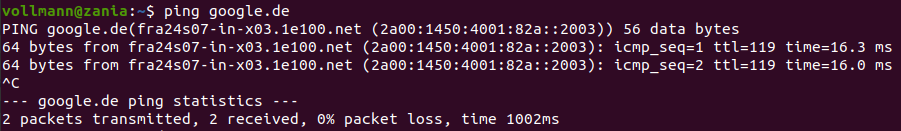
\includegraphics[width=0.7\linewidth]{./media/ping_google}
		\caption[\texttt{ping} an Google]{\texttt{ping} an www.google.de.}
		\label{fig:pinggoogle}
	\end{figure}
\end{itemize}

\demo{
\begin{itemize}
	\item \ttt{ssh syrma.uni-trier.de}
	\item \ttt{rsync} remote (e.g. \ttt{ssh syrma.uni-trier.de}) to local
	\item \ttt{ping}
\end{itemize}
}
\homework{\textbf{Hausaufgaben}
\begin{enumerate}
	\item Welche Verbindungsart nutzen Sie gerade, um ins Internet zu kommen?
	\item Welche IP-Adresse hat Ihr Gerät gerade?
	\item Wurde diese IP-Adresse statisch oder dynamisch vergeben?
\end{enumerate}
}
\inclass{
	\textbf{Analysieren Sie Ihr Heimnetz}
	\begin{itemize}
		\item Welche VRs (zB Router, Repeater, Powerlink) sind vorhanden?
		\item Welche netzwerkfähigen Geräte sind in Ihrem Heimnetz? Rechner, TV, Smartphone, Synology/NAS/, Heizung, Drucker, Herdplatte, Lampen, Fahrrad-Tacho,...
		\item Wie sind diese Geräte miteinander verbunden (\textit{wire(less)})? Welches Protokoll verwenden Ihre Geräte im WLAN? Was ist eigentlich ein WLAN-Schlüssel?
		\item Finden Sie heraus, welche IP-Adresse Ihr Rechner oder Smartphone von Ihrem Router aktuell zugeordnet bekommen hat. Wie lautet die Netzadresse? Geben Sie diese Netzadresse in Google ein: Was ist die Besonderheit dieser Netzadresse (Stichwort: Private IP-Adresse)?
		\item Falls Sie Zugang haben sollten: Schauen Sie sich auch mal in der Browser-Maske Ihres Routers um (zB \url{http://fritz.box/}). Welche Internetadresse hat Ihr Router (Freigaben festgelegt für Erreichbarkeit von außen)?\\
		Meiner besitzt (aktuell) als Netzadressen-Anteil: \texttt{217.251} mit Gateway \link{https://ipinfo.io/217.251.34.1}{\texttt{217.251.34.1}}, ein Gateway in Trier von der Deutsche Telekom AG
		\item Falls Sie Zugang haben sollten: Können Sie Ihren Geräte feste IPs zuweisen? Zum Beispiel sinnvoll, um den eigenen Netzwerk-Drucker stets unter der selben IP zu erreichen.
			\item Schauen Sie in ihrem Dateimanager nach den Optionen nfs://, smb://, sftp://, ftp://, dav://
	\end{itemize}
}


\clearpage
\subsection{Virtualisierung}
\link{https://de.wikipedia.org/wiki/Virtualisierung_(Informatik)}{\textbf{Virtualisierung}}\footnote{``Virtuell'' wie ``nicht-physisch''} bezeichnet in der Informatik die Nachbildung (Emulation) eines Hard- oder Software-Objekts durch ein ähnliches Objekt vom selben Typ mit Hilfe einer \textbf{Abstraktionsschicht}.
~\\~\\
Zur Unterscheidung echter und virtueller Umgebungen werden diese  Wirt (\textit{host}) und Gast (\textit{guest}) genannt:
\begin{itemize}
	\item \textbf{Wirt} (\textit{host}): bezeichnet immer die Ebene (oder Schicht), welche der physischen Hardware am nächsten ist
	\item \textbf{Gast} (\textit{guest}): die auf dem Wirt ausgeführte Umgebung
\end{itemize}
~\\
\textit{Anwendungsbeispiel:} Betriebssystem innerhalb eines anderen ausführen.
\begin{itemize}
	\item Mithilfe einer geeigneten Virtualisierer-Software (zB Virtualbox oder VMWare) können wir beispielsweise andere Betriebssysteme (zB Gast = Ubuntu 20.04) in einem Fenster unter unserem derzeitigen Betriebssystem (zB Host = Windows 10) nutzen und Dateien zwischen Host- und Gast-Betriebssystem austauschen.
\item Dabei \textit{emuliert} die Virtualisierer-Software die fehlende PC-Hardware des virtuellen Betriebssystems und leitet Hardware-Anfragen an die echte Hardware (CPU, Grafikkarte, Festplatte) des physisch vorhandenen PCs weiter.
\item Es wird dem Gast-Betriebssystem die Alleinnutzung eines Computers vorgegaukelt, wobei es tatsächlich innerhalb eines anderen Betriebssystems als gewöhnliche Anwendung läuft.
%\item Letztlich wird so ein Betriebssystem \textit{simuliert}, dessen Hardware aber \textit{emuliert} ist.
\end{itemize}
%
\textit{Weitere Anwendungsbeispiele und Vorteile:}
\begin{itemize}
	\item Computer-Ressourcen/Dienste aufteilen oder zusammenfassen
	\item Agilität durch \textbf{Unabhängigkeit} von der physischen Hardwareinfrastruktur\\
	$\to$ Abstraktionsschicht täuscht (andere) physische Gegebenheiten vor
	\item Agilität durch \textbf{Modularisierung} (eine virtuelle Machine bekommt nur eine einzige Aufgabe; kann schnell ausgetauscht werden)
\end{itemize}
\demo{
\begin{itemize}
	\item Fallbeispiel: Mathe-Netz (abstrakt und proxmox)
\end{itemize}
}
~\\
Wir schauen uns in diesem Zusammenhang noch kurz etwas um:
\begin{itemize}
	\item Softwarevirtualisierung: Virtuelle Maschinen und Container
	\item Hardwarevirtualisierung
	\item Netzwerkvirtualisierung: VLAN und VPN
\end{itemize}






\subsubsection{Softwarevirtualisierung}
Wir unterscheiden: Virtuelle Maschinen und Container.\\
~\\
\textbf{Virtuelle Maschine: Systemvirtualisierung mittels Hypervisor}\\
Als virtuelle Maschine (VM) wird in der Informatik die Software-technische Kapselung eines Rechnersystems innerhalb eines lauffähigen Rechnersystems bezeichnet.
\begin{itemize}
	\item Das Betriebssystem der VM verwendet dabei seinen eigenen Betriebssystemkern.
	\item Die Abstraktionsschicht zwischen Host und Gast wird \textbf{Hypervisor} oder \textbf{Virtual Machine Monitor} genannt.
	\item Bekannte Umsetzungen:
	\begin{itemize}
		\item Oracles \link{https://de.wikipedia.org/wiki/VirtualBox}{VirtualBox},
		\item VMwares \link{https://de.wikipedia.org/wiki/VMware_vSphere}{vSphere}.
	\end{itemize}
\end{itemize}
~\\~\\
\textbf{Container: Systemvirtualisierung mittels OS-Container}\\
\link{https://de.wikipedia.org/wiki/Containervirtualisierung}{Containervirtualisierung} (oder Containering) ist eine Methode, um mehrere Instanzen eines Betriebssystems (als Gäste) isoliert voneinander den Kernel des Hosts nutzen zu lassen.

\begin{itemize}
	\item Im Gegensatz zur Virtualisierung mittels eines Hypervisors gilt Containervirtualisierung als besonders ressourcenschonend.
	\item Containern (Sandbox) haben nur Zugriff auf einen Teil der \textbf{Systemressourcen:}
	\begin{itemize}
		\item Nutzbare Hardware(komponenten), wie CPU und Netzwerk
		\item Speicher (Lesen/Schreiben), Ordnerstrukturen und Netzwerkspeicher
		\item Peripheriegeräte wie Tastatur, Webcam, Scanner und Drucker.
	\end{itemize}
	\item Bekannte Umsetzungen:
	\begin{itemize}
		\item \link{https://de.wikipedia.org/wiki/LXC}{\textbf{LXC}} (Linux Container)
		\item \link{https://de.wikipedia.org/wiki/Docker_(Software)}{\textbf{Docker}}; benutzerfreundliche Werkzeuge (u.a. eine Beschreibung von Images (Dockerfiles) oder ein Repository, das solche Images verwaltet); seit ca. 2013 sehr populär.
	\end{itemize}
\end{itemize}


\inclass{
%	\textbf{Wer Lust hat:}\\
	~\\
	\textbf{VMs}
	\begin{enumerate}
		\item VirtualBox installieren (gui): \url{https://www.virtualbox.org/wiki/Downloads}
		\item Ubuntu 20.04 als VM installieren
		\item Ggf müssen Sie Virtualisierung auf Ihrer CPU zunächst erlauben:\\
		Enable Virtual Hardware in BIOS/UEFI.\\
		Press F2 (or other F- ..) key at startup BIOS/UEFI Setup.\\
		Switch to the Advanced Mode tab then choose CPU Configuration option.\\
		Scroll down to the ''Intel Virtualization Technology'' value, and then change [Disabled]->[Enabled].\\
		Save Changes and Exit.
	\end{enumerate}
~\\
\textbf{Container}
\begin{enumerate}
	\item docker desktop/server installieren; siehe \url{https://docs.docker.com/engine/install/}
	\item Von Docker Hub ein Docker Image (instanz) ausführen; zB nextcloud (\url{https://hub.docker.com/_/nextcloud})
\end{enumerate}
}

\subsubsection{Hardwarevirtualisierung}
Hierfür können entweder das ganze System oder nur einzelne seiner Komponenten, wie z.B. CPU oder GPU, virtualisiert werden.\\~\\ \textit{Anwendungsbeispiel:} GPU eines leistungsfähigen GPU-Servers virtuell partitionieren und Anwendern (zB Studierenden) diese für einen gewissen Zeitraum (zB Abschlussarbeit) für rechenintensive Probleme isoliert zur Verfügung stellen.

\subsubsection{Netzwerkvirtualisierung}
Durch die physikalisch angeklemmte Hardware entsteht über Router, Switches, Rechner, Drucker etc. ein physikalisches Netzwerk (zB innerhalb der Uni).\\~\\
\textbf{Virtual Local Area Network (VLAN)}\\
Um das Netzwerk in einzelne Teilbereiche (sog. Subnetze) \textit{unabhängig von der phsysischen Gegebenheit} zu unterteilen, bedarf es einer geeigneten Virtualisierung. Damit bleibt man auch hier agil und flexibel. Ein \link{https://de.wikipedia.org/wiki/Virtual_Local_Area_Network}{Virtual Local Area Network (VLAN)} ist ein logisches Subnetz welches sich über mehrere Switches hinweg ausdehnen kann.\\~\\
\textit{Anwendungsbeispiel:} Das Netz der Universität Trier kann folgende IPs vergeben $$\texttt{136.199.XXX.YYY}.$$ Dabei können feste Zahlen \texttt{XXX} als Subnetze/VLANs verstanden werden, in denen dann 256 verschiedene IPs für Rechner, Drucker, Server etc vergeben werden können. Zum Beispiel betreiben wir in der Mathematik die Subnetze:
\begin{itemize}
	\item \texttt{136.199.123.YYY} (Mitarbeiter selbst verwaltet),
	\item \texttt{136.199.234.YYY} (Mitarbeiter zentral verwaltet, CIP Pools),
	\item \texttt{136.199.235.YYY} (www-Server),
	\item \texttt{136.199.236.YYY} (Testwiese).
\end{itemize}
Durch geeignete Firewall-Regeln kann zudem der Zugriff aus und auf die Subnetze geregelt werden. So sollte zum Beispiel ein Web-Server im Subnetz \texttt{136.199.235.YYY} nach außen sichtbar sein und http(s)-Anfragen o.ä. von beliebigen IP-Adressen beantworten. Auf Knoten im Mitarbeiter-Netz \texttt{136.199.234.YYY} können hingegen nur einige priviligierte IP-Adressen außerhalb der Range \texttt{136.199.234.YYY} zugreifen.
~\\~\\
\textbf{Virtual Private Network (VPN)}\\
Andererseits möchte man auch über Knoten (wie Router, Switches,..), die nicht im eigenen Hardwarebestand sind, ein geschütztes isoliertes Netz administrieren (zB das Netz der Universität Trier; Unternehmsnetz).\\~\\ Ein \link{https://de.wikipedia.org/wiki/Virtual_Private_Network}{Virtual Private Network} (VPN) bildet ein nach außen abgeschirmtes Netzwerk über fremde oder nicht vertrauenswürdige Netze. Virtuell in dem Sinne, dass es sich nicht um eine eigene physische Verbindung handelt, sondern um ein bestehendes Kommunikationsnetz, das als Transportmedium verwendet wird.\\
~\\
\textit{Anwendungsbeispiel:}
\begin{itemize}
	\item Der Computer eines Studierenden kann von zu Hause aus Zugriff auf das Uni-Trier-Netz erlangen. Aus Sicht der VPN-Verbindung dienen die dazwischen liegenden Netze (sein Heimnetz sowie das Internet) als Verlängerungskabels, das den Computer (VPN-Partner) ausschließlich mit dem zugeordneten Netz verbindet (VPN-Gateway).
\item Der sich daraus ergebende Nutzen eines VPNs kann je nach verwendetem VPN-Protokoll durch eine Verschlüsselung ergänzt werden, die eine abhör- und manipulationssichere Kommunikation zwischen den VPN-Partnern ermöglicht.
\item Ein verschlüsseltes VPN über ein unverschlüsseltes Netzwerk herzustellen, ist mit eine der Hauptgründe für die Verwendung eines VPNs.
\end{itemize}
Sobald ein Computer eine VPN-Verbindung aufbaut, ist der Vorgang vergleichbar mit dem Umstecken seines Netzwerkkabels von seinem ursprünglichen Netz an das neu zugeordnete Netz, mit allen Auswirkungen wie geänderten IP-Adressen und Unterschieden beim Routing.

\inclass{
	\textbf{Eigenes VPN}
	\begin{itemize}
		\item Wer Lust und Zeit hat: VPN Heimnetz konfigurieren mithilfe ihres Routers, zB fritz.box. Damit könnten Sie zB von unterwegs mittels ihres Smartphones über das Internet (LTE, ...) getunnelt einen Druckauftrag o.ä nach Hause senden oder ihre eigene Nextcloud (die sie zuvor einfach als Docker image installiert haben) erreichen.
	\end{itemize}
}

\homework{\textbf{Hausaufgabe:
		\begin{center}
		\large	VPN + Anmeldung auf dem Remote Server
	\end{center}}
\begin{enumerate}
	\item Verschaffen Sie sich Zugang zum VPN der Universität Trier über Ihre ZIMK-Kennung.
	\item Melden Sie sich auf dem Server \remoteServer\ an. [Siehe Anleitung auf der Titelseite.]
\end{enumerate}
}
